% Auriga theme
% find the most up-to-date version here: https://github.com/anishathalye/auriga

% \documentclass[14pt,aspectratio=169]{beamer}
\documentclass[9pt]{beamer}
\usepackage[T1]{fontenc}
\usepackage{lmodern}
\usetheme{auriga}
\usecolortheme{auriga}
\usepackage{graphicx}
\usepackage{xcolor}
\usepackage{wrapfig}

\usepackage{tikz}
\usetikzlibrary{arrows,arrows.meta,shapes, decorations.pathmorphing,decorations.markings,backgrounds,calc,positioning}
\usetikzlibrary{overlay-beamer-styles}

\usepackage{pgfplots}
\pgfplotsset{compat=1.14}

\usepackage{amssymb,amsfonts,amsmath,mathtext}
\usepackage{color,enumerate,float,indentfirst}
\usepackage{caption, subcaption}
% \usepackage{environ}
\usepackage{tcolorbox}
\usepackage{geometry}
\usepackage{pdfpages}

\usepackage{biblatex}
\addbibresource{refs.bib}

\usepackage[symbol]{footmisc}

% for notes
% \setbeamertemplate{note page}{\pagecolor{yellow!5}\insertnote}
% \setbeameroption{show notes on second screen=right}

% \usetikzlibrary{shadows}
\usepackage{soul}
\usepackage{lipsum}

% \usefonttheme{professionalfonts}

\newtheorem{ttheorem}{Теорема}
\renewcommand{\thefootnote}{\fnsymbol{footnote}}

\setbeamercolor{footline}{fg=blue}

% define some colors for a consistent theme across slides
\definecolor{red}{RGB}{181, 23, 0}
\definecolor{blue}{RGB}{0, 118, 186}
\definecolor{gray}{RGB}{146, 146, 146}

% some tikz parameters
\tikzset{
mystyle/.style={
  circle,
  line width=1pt,
  inner sep=0pt,
  text width=3.5em,
  align=center,
  draw=black,
  }
}
\tikzset{
myline/.style={
  line width=0.7pt,
  -{Latex[length=3mm]}
  }
}
\tikzset{
mysnake/.style={
  decoration={snake, pre length=0.01mm, segment length=2mm, amplitude=0.3mm, post length=3mm},
  decorate
  }
}

\newcommand{\itemi}{\item[\checkmark]}

\begin{document}

\title{Объектно-центричное представление мира агента в обучении с подкреплением}

\author{%
    \textbf{Студент:}~Ярослав Ивченков \inst{1} \\
    \textbf{Научный руководитель:}~Матвеев И. А.,~д.т.н. \inst{1} 
}

\institute[shortinst]{%
    \inst{1} Московский Физико-Технический Институт \samelineand 
    \inst{2} Научно-Исследовательский Институт Искусственного Интеллекта (AIRI)
}

\titlegraphic{
    % \begin{figure}
    %     \begin{subfigure}{.8\textwidth}
    %         \centering
    %         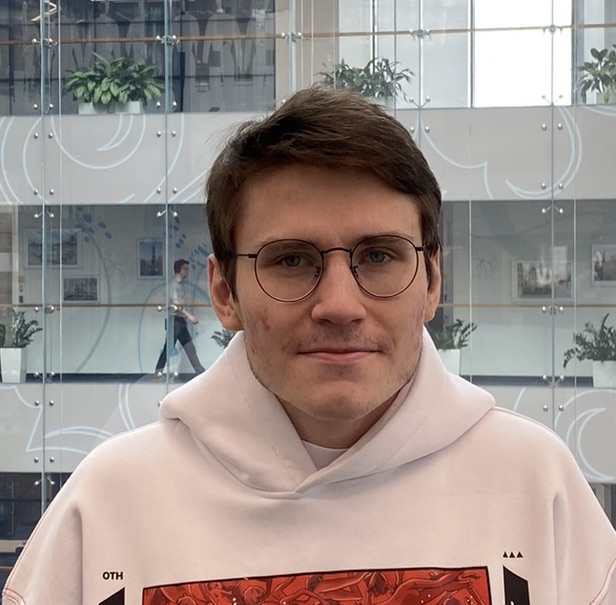
\includegraphics[height=2cm]{images/authors/ivchenkov_yaroslav.jpeg}
    %         \centering
    %         \hspace{2em}
    %         
\includegraphics[height=2cm]{images/authors/panov_aleksandr.png}
    %     \end{subfigure}
    % \end{figure}
    \begin{figure}
        \begin{subfigure}{.45\textwidth}
            \raggedleft
            
\includegraphics[height=1.5cm]{images/logos/mipt.png}
        \end{subfigure}
        \begin{subfigure}{.45\textwidth}
            \raggedright
            
\includegraphics[height=0.8cm]{images/logos/airi_dark.png}
        \end{subfigure}
    \end{figure}
    %\parbox[c]{3cm}{
\includegraphics[height=2cm]{images/logos/mipt.png}}
    %\hspace{0.75cm}%
    %\parbox[c]{4cm}{
\includegraphics[height=1.15cm]{images/logos/airi_dark.png}}
}

\setbeamercolor{page number in head/foot}{fg=background canvas.bg}
\begin{frame}
\titlepage
\end{frame}
\note{Hello, my name is Yaroslav and I'm presenting Factorized World Models for Learning Causal Relationships. This is joint work with Artem Zholus from Moscow Institute of Physics and Technology and Aleksandr Panov from Artificial Intelligence Research Institute.\\
\textasciitilde 15s}

% \setbeamercovered{transparent}
\begin{frame}{Cause-Effect Modeling Agent}
% TODO: make them appear and disappear as in slides
\begin{itemize}
    \item<1-> Structured World Model capable of OOD task generalisation in visual control tasks
    \note[item]<1->{We want to present Cause-Effect Modeling Agent, in short CEMA, the Model-Based Reinforcement Learning Agent with Structured World Model, designed for solving Out-Of-Distribution tasks in visual control setting}
    \item<2-> Learning causal invariance of a robot influencing changes of the object state
    \note[item]<2->{CEMA is able to learn causality between changes in robot state and changes in object state.}
    \item<3-> Latent state factorization into robot and object states given segmentation
    \note[item]<3->{World Model takes as input segmented images of environment and its latent state is factored into robot and object states.}
    \item<4-> Different dynamics models of robot and object with influence vector as link
    \note[item]<4->{Both actor and object have their own dynamics connected via influence vector}
\end{itemize}
    
\end{frame}
\setbeamercovered{invisible}
\begin{frame}
\frametitle{Постановка задачи}
\begin{itemize}
    \item Среда: Марковский Процесс Принятия Решений $\left<S, A, R, p, \gamma\right>$
    \begin{itemize}
        \item $S$ -- пространство состояний
        \item $A$ -- пространство действий
        \item $p(s'\mid s, a)$ -- функция перехода состояний среды
        \item $R(s, s', a)$ -- функция вознаграждения среды
    \end{itemize}
    \item Задача: найти стратегию $\pi(a\mid s)$ максимизирующую ожидаемую отдачу $J(\pi, p, R) = \mathbb{E}_{p, \pi} \sum_t \gamma^t R_t$
    \item Модельное обучение с подкреплением: аппроксимировать функцию перехода состояний среды и функцию награды ``моделью мира'' $\hat{p}_{\theta}(s'\mid s, a)$, $\hat{R}_{\theta}(s, s', a)$ с которой агент может взаимодействовать с целью максимизации $J(\pi, \hat{p}_{\theta}, \hat{R}_{\theta})$. Модель мира обучается на буфере опыта, полученного из взаимодействия агента со средой.
    \item Обобщение между задачами: пусть дано распределение задач (каждая из которых является МППР) $p_{\text{train}}(\tau)$. Обучая модельного агента на задачах $\tau \in p_{\text{train}}(\tau)$, необходимо максимизировать ожидаемую отдачу на задачах $\tau \in p_{\text{test}}(\tau)$.
\end{itemize}
\end{frame}
\setbeamercovered{transparent}
\begin{frame}{Объектно-центричное обучение}
    \begin{itemize}
        \item<1-4> Базовое предположение: наблюдение состоит из $N$ объектов, каждый из которых может быть смоделирован по отдельности
        \item<2-4> Объекты могут взаимодействовать друг с другом и влиять друг на друга
        \item<3-4> Объектная абстракция позволяет ввести структуру в наблюдения, представленные изображениями в таких задачах, как предсказание видео или визуальный контроль в обучении с подкреплением
        \item<4> Может быть применено для повышения скорости обучения и обобщающих способностей в обучении с подкреплением
    \end{itemize}
    
\end{frame}
\setbeamercovered{invisible}

% \begin{frame}{Object-Centric Learning with Slot Attention \cite{SlotAttention}, NIPS'20 }
%     \begin{columns}
%     \begin{column}{0.7\textwidth}
%     \begin{itemize}
%         \item Object-centric approach to representation learning
%         \item Main contribution - Slot Attention module
%         \item Maps $N$ input feature vectors to $K$ \textit{slots}
%     \end{itemize}
%     \end{column}
%     \begin{column}{0.4\textwidth}
%     \begin{figure}
%         \centering
%         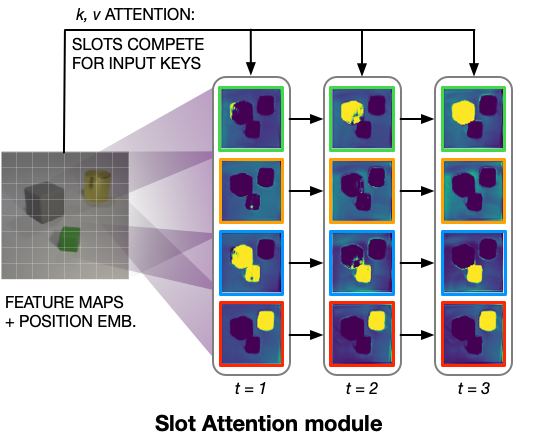
\includegraphics[width=\linewidth]{images/rel_work/slot_att_scheme.png}
%         % \caption{Slot Attention Scheme}
%         % \label{fig:slot_att}
%     \end{figure}
%     \end{column}
%     \end{columns}
% \end{frame}

% \begin{frame}{Object-Centric Learning with Slot Attention \cite{SlotAttention}, NIPS'20}
%     \begin{columns}
%     \begin{column}{0.45\textwidth}
%     Applications:
%     \begin{itemize}
%         \item Unsupervised object discovery
%         \begin{itemize}
%             \item Number of slots is hyperparameter
%         \end{itemize}
%         \item Set prediction
%         \begin{itemize}
%             \item Sets are predicted with MLP
%         \end{itemize}
%     \end{itemize}
%     \begin{figure}
%         \centering
%         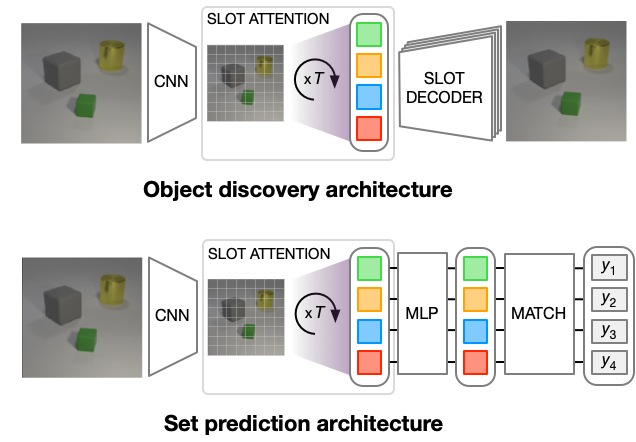
\includegraphics[width=\linewidth]{images/rel_work/slot_att_arch.png}
%         % \caption{Object detection experiment}
%         % \label{fig:slot_att_obj_detect}
%     \end{figure}
%     \end{column}
    
%     \begin{column}{0.45\textwidth}
%     \begin{figure}
%         \centering
%         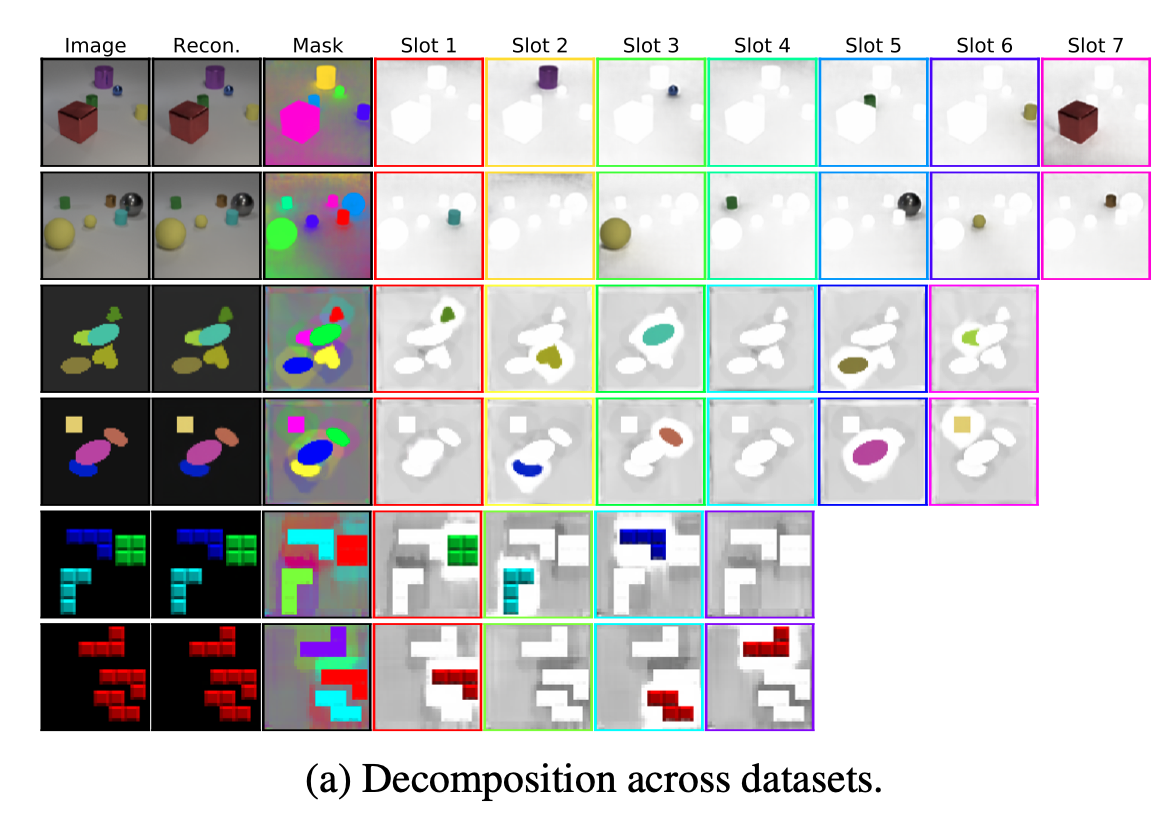
\includegraphics[width=\linewidth]{images/rel_work/slot_att_obj_recogn.png}
%         % \caption{Object detection experiment}
%         % \label{fig:slot_att_obj_detect}
%     \end{figure}
%     \end{column}
%     \end{columns}
% \end{frame}

% \begin{frame}{Contrastive Learning of Structured World Models \cite{cSWM}, ICLR'20}
%     \begin{itemize}
%         \item Both action and state spaces are factorized
%         \item Transition model is message-passing GNN
%         \item Multi-object contrastive learning using samples from buffer
%     \end{itemize}
%     \begin{figure}
%         \centering
%         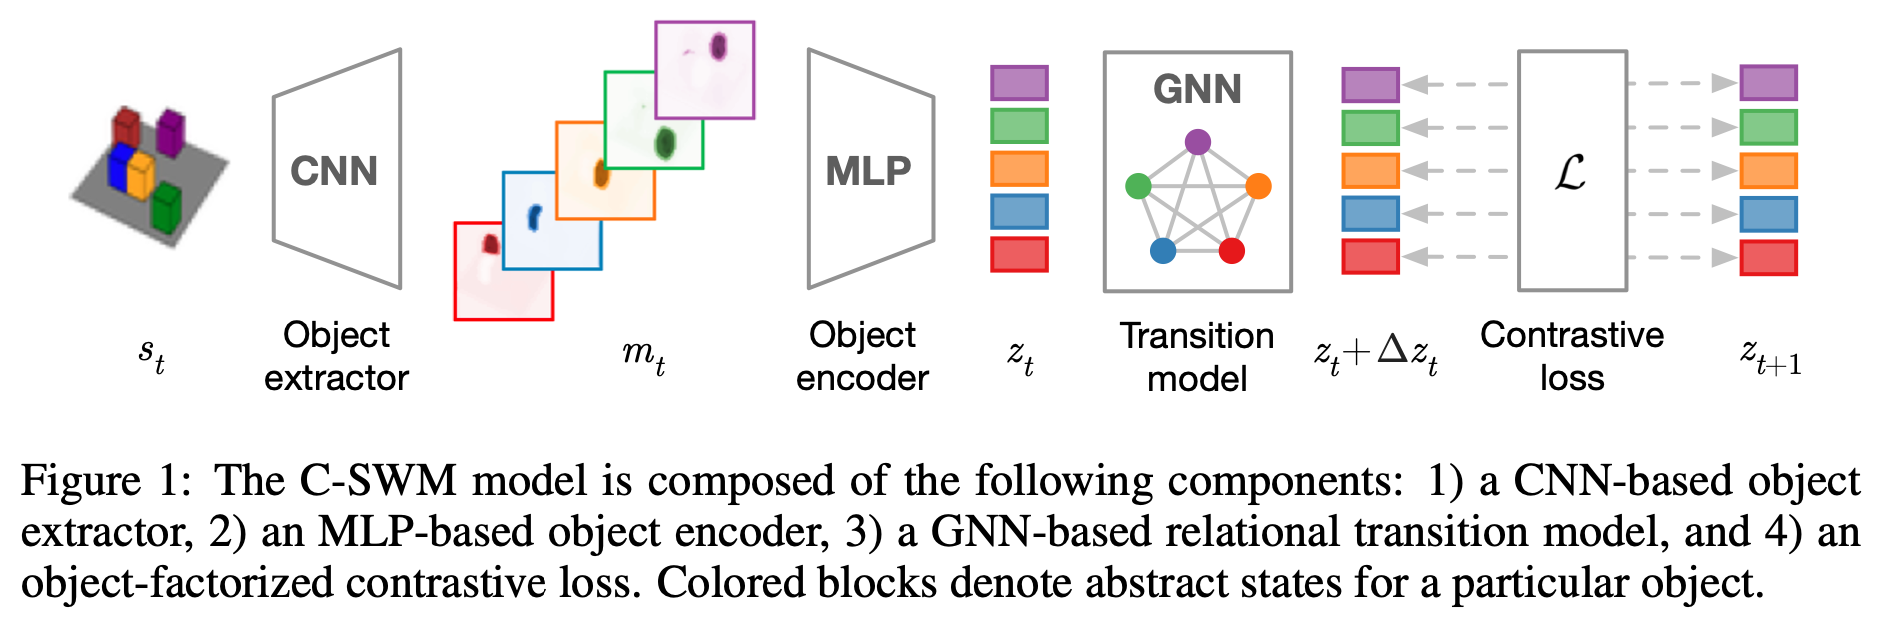
\includegraphics[height=0.3\paperheight]{images/rel_work/cswm_scheme.png}
%         % \caption{C-SWM scheme}
%         % \label{fig:cswm_scheme}
%     \end{figure}
% \end{frame}
% \begin{frame}{Contrastive Learning of Structured World Models \cite{cSWM}, ICLR'20}
%     Experiments:
%     \begin{itemize}
%         \item Multiple environments with different moving objects
%         \item Atari Pong and Space Invaders
%         \item Objective - predict the next observation after taking the action/actions.
%     \end{itemize}
%     \begin{figure}
%         \centering
%         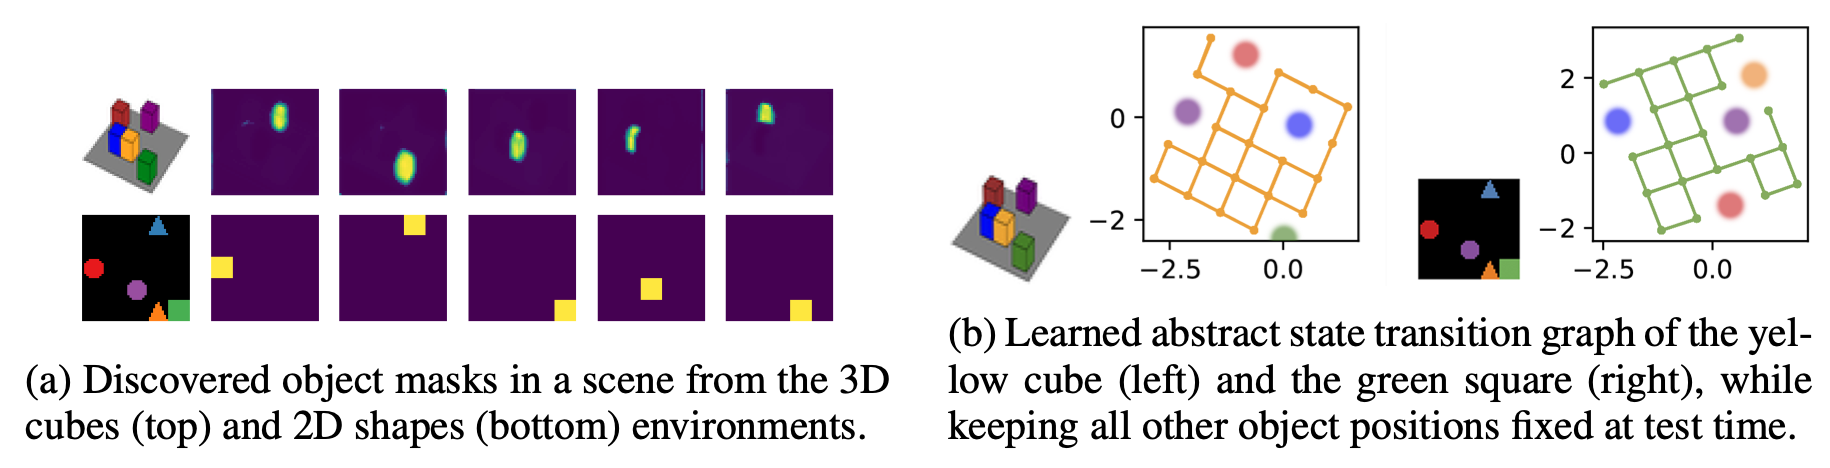
\includegraphics[height=0.3\paperheight]{images/rel_work/cswm_predictions.png}
%         % \caption{CSWM experiment results}
%         % \label{fig:my_label}
%     \end{figure}
% \end{frame}

% \begin{frame}{Entity Abstraction in Visual Model-Based Reinforcement Learning \cite{OP3}, CoRL'19}
%     \begin{itemize}
%         \item Generalization via modeling universal interaction and entities
%         \item Designed for combinatorical tasks with similar objects
%         \item Can be applied for goal-conditioned RL and object detection in videos
%     \end{itemize}
%     \begin{figure}
%         \centering
%         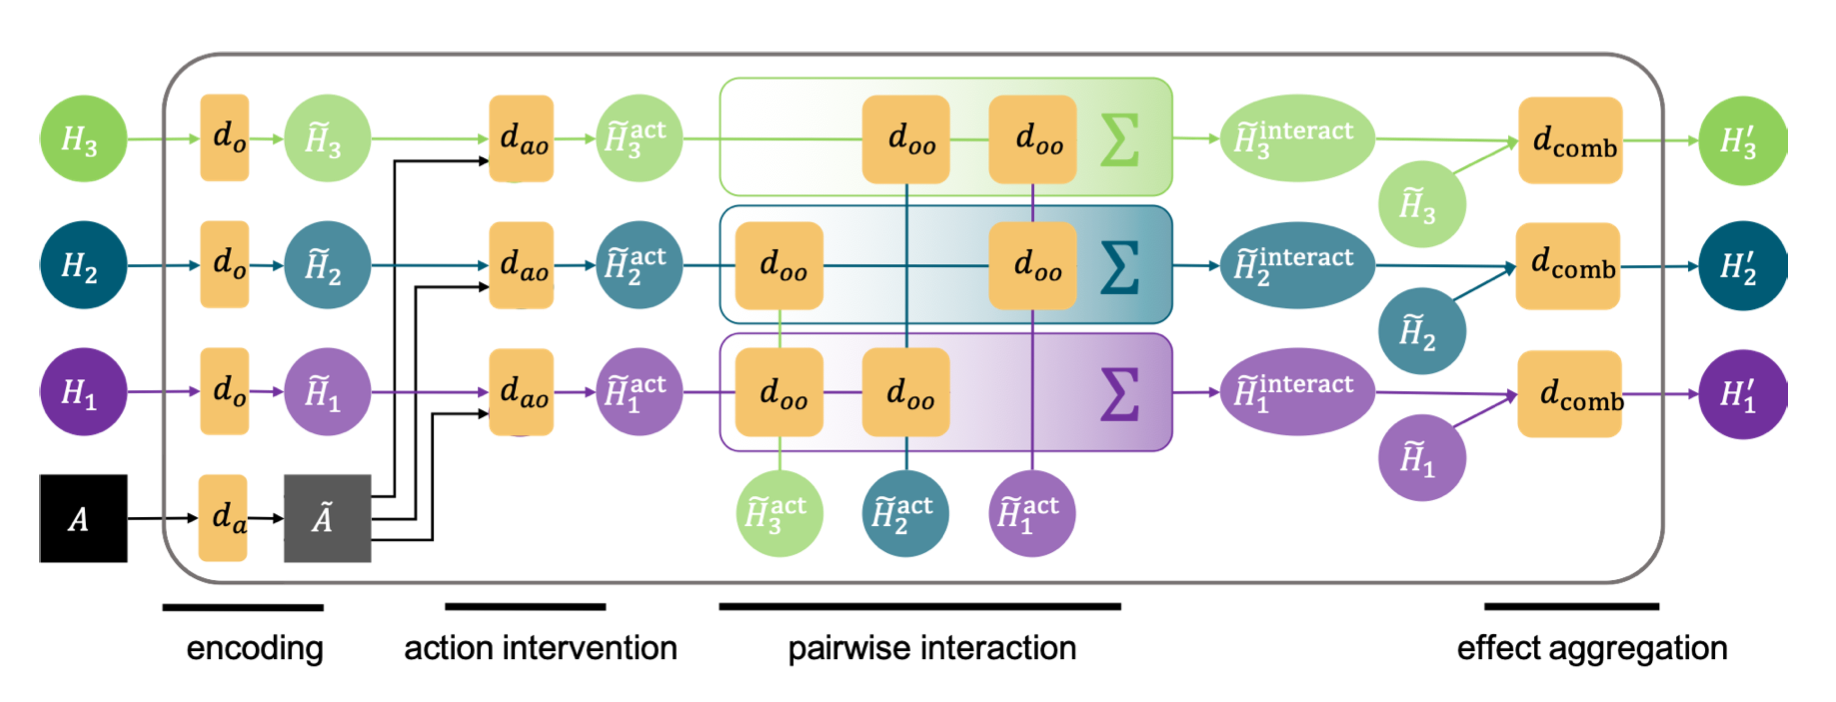
\includegraphics[height=0.3\paperheight]{images/rel_work/op3_dynamics.png}
%         % \caption{ROLL scheme}
%         % \label{fig:roll_scheme}
%     \end{figure}
% \end{frame}

% \begin{frame}{GATSBI: Generative Agent-centric Spatio-temporal Object Interaction \cite{GATSBI}, CVPR'21}
% \begin{columns}
% \begin{column}{0.45\textwidth}
%     \begin{itemize}
%         \item Unsupervised spatio-temporal representation
%         \item Three entity categories
%         \item GMM for grounding large components
%         \item Keypoint module for robot, attention-based object module
%         \item Interactions as GNN consider different nature of objects
%     \end{itemize}
% \end{column}
% \begin{column}{0.45\textwidth}
%     \begin{figure}
%         \centering
%         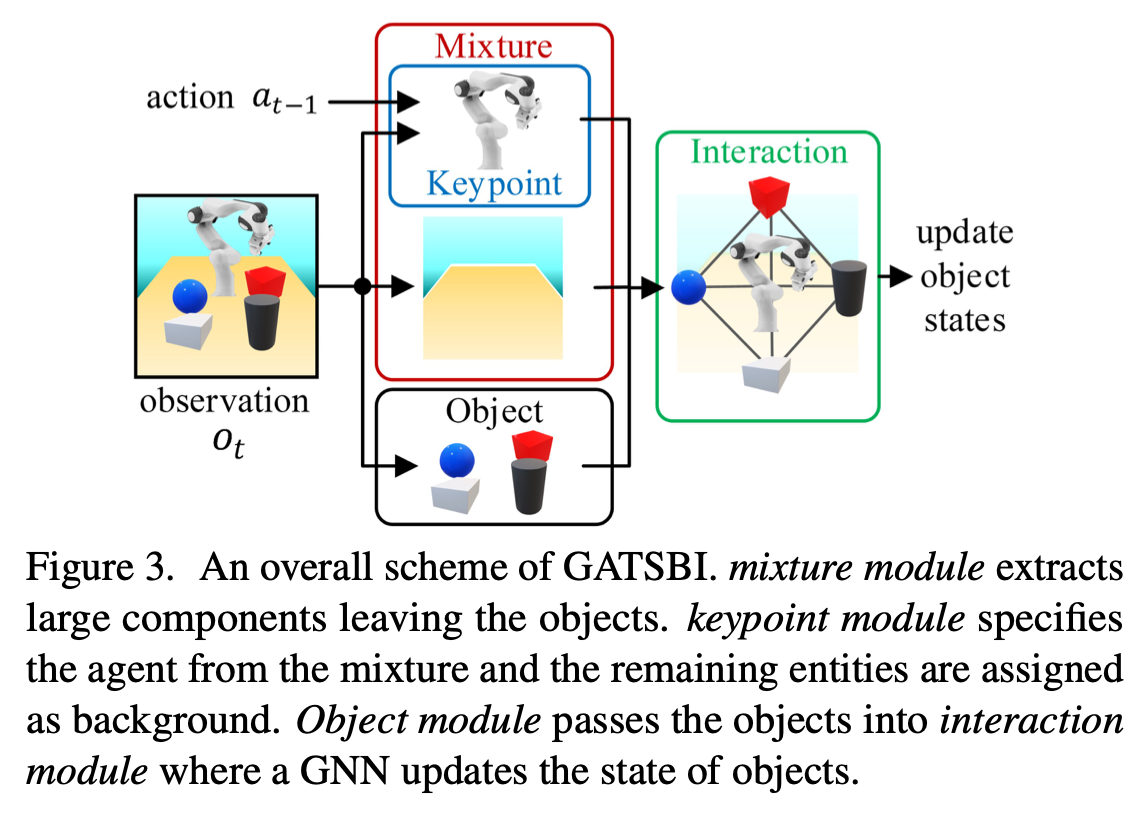
\includegraphics[width=\linewidth]{images/rel_work/gatsbi_scheme.png}
%         % \caption{ROLL scheme}
%         % \label{fig:roll_scheme}
%     \end{figure}
% \end{column}
% \end{columns}
% \end{frame}

% \begin{frame}{ROLL: Visual Self-Supervised Reinforcement Learning with Object Reasoning \cite{ROLL}, CoRL'20}
% \begin{columns}
% \begin{column}{0.45\textwidth}
%     \begin{itemize}
%         \item Object-centric approach to goal-conditioned RL
%         \item Explicitly segmented robot, background and objects
%         \item Deals with occluded objects
%     \end{itemize}
% \end{column}
% \begin{column}{0.45\textwidth}
%     \begin{itemize}
%         \item Works under assumptions that background is static and reward depends on the object position
%         \item Most of the training performed offline
%     \end{itemize}
% \end{column}
% \end{columns}
% \begin{figure}
%     \centering
%     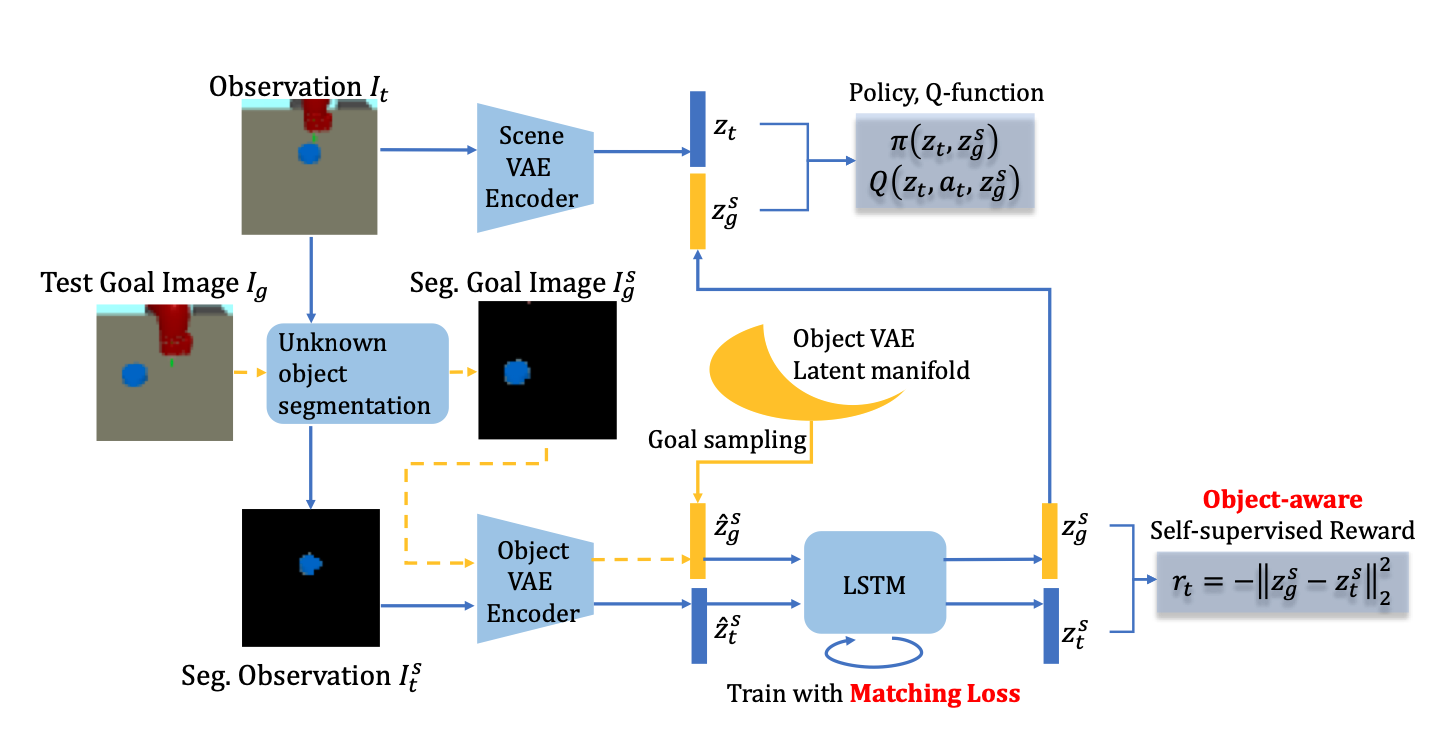
\includegraphics[height=0.4\paperheight]{images/rel_work/roll_scheme.png}
%     % \caption{ROLL scheme}
%     % \label{fig:roll_scheme}
% \end{figure}
% \end{frame}

% \begin{frame}{CAI \cite{CAI}, NIPS'21}
%     \begin{itemize}
%         \item Causal Influence Detection for Improving Efficiency in RL
%         \item Interactions as causal graph
%         \item Control is quantified and measured
%         \item Applications to RL:
%         \begin{itemize}
%             \item Reward bonus for Causal Action Influence (CAI)
%             \item Exploratory policy using CAI
%             \item Causal Influence-based Experience Replay
%         \end{itemize}
%     \end{itemize}
%     \begin{figure}
%         \centering
%         \includegraphics[height=0.3\paperheight]{images/rel_work/causal_scheme.png}
%         % \caption{ROLL scheme}
%         % \label{fig:roll_scheme}
%     \end{figure}
% \end{frame}
\setbeamercovered{transparent}
\begin{frame}
\frametitle{Comparison}
    Differences:
    \begin{itemize}
        \item<1-5> Presence of temporal context
        \item<2-5> Presence of conditional factors
        \item<3-5> Entity categories
        \item<4-5> Interaction model
        \item<5> Particular task peculiarities
    \end{itemize}
\end{frame}
\setbeamercovered{invisible}
\begin{frame}
\frametitle{Объектно Центричный Визуальный Контроль}

\begin{columns}[t]
\begin{column}{0.43\linewidth}
    Обычная задача визуального контроля включает в себя:
    \begin{itemize}
        \item Актуатор, напрямую контролируемый действиями
        \item Объекты, косвенно контролируемые актуатором
        \item Функцию награды, подразумевающую взаимодействие между актуатором и объектом(-ами).
    \end{itemize}
\end{column}

\begin{column}{0.55\linewidth}
    \begin{figure}
    \centering
    \begin{subfigure}[c]{.45\linewidth}
        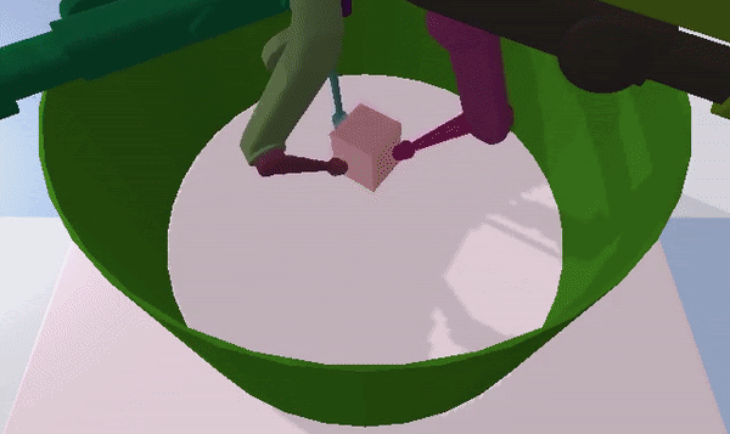
\includegraphics[width=\linewidth]{images/visual_control_envs/causal_world.png}
    \end{subfigure}
    \hspace{1em}
    \begin{subfigure}[c]{.45\linewidth}
        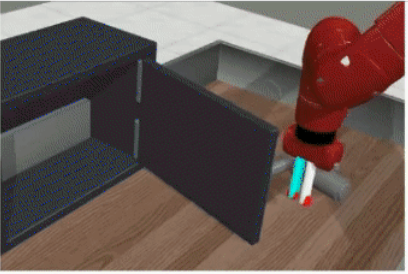
\includegraphics[width=\linewidth]{images/visual_control_envs/metaworld.png}
    \end{subfigure}
    \vspace{3em}
    
    \begin{subfigure}[c]{.45\linewidth}
        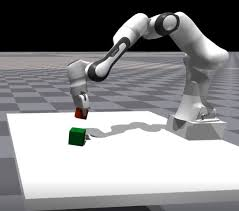
\includegraphics[width=\linewidth]{images/visual_control_envs/isaac_gym.jpeg}
    \end{subfigure}
    \hspace{1em}
    \begin{subfigure}[c]{.45\linewidth}
        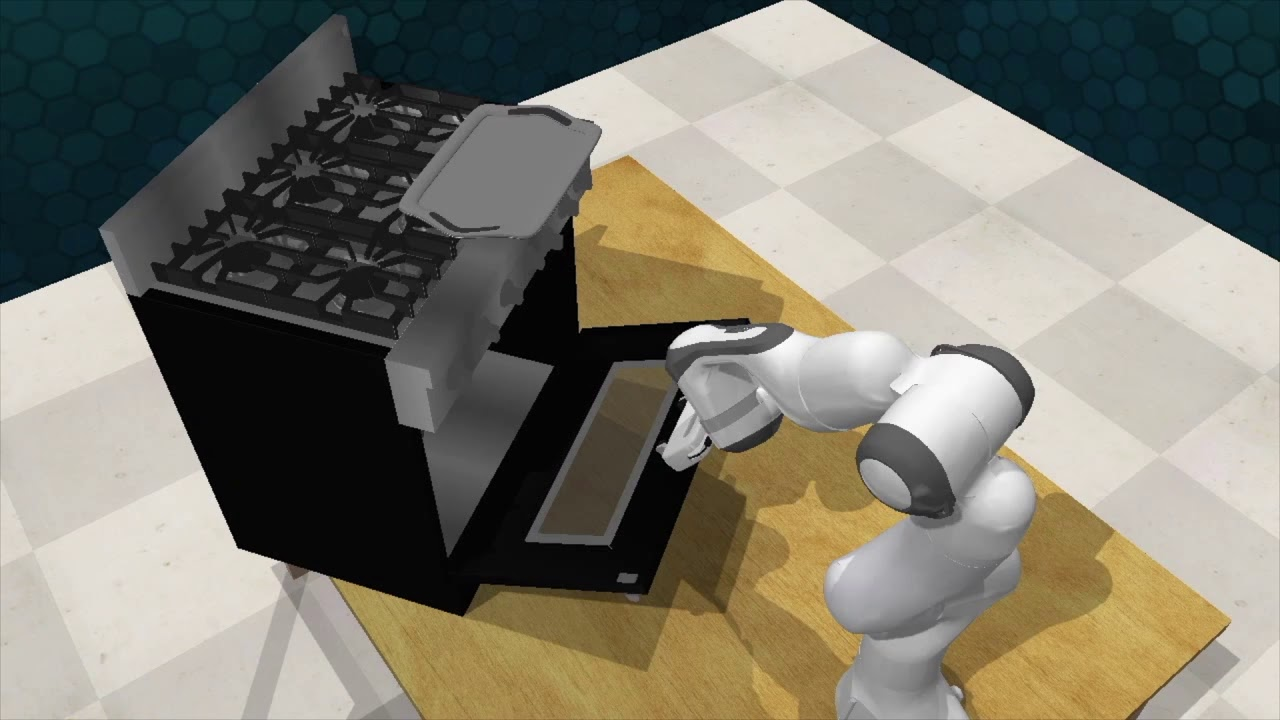
\includegraphics[width=\linewidth]{images/visual_control_envs/rl_bench.jpg}
    \end{subfigure}
    \caption{Различные среды визуального контроля}
    \end{figure}
\end{column}
\end{columns}

% \begin{minipage}[t]{0.48\linewidth}
%     Typical visual control environment:
%     \begin{itemize}
%         \item Directly controlled actuator
%         \item Success implies interaction between actuator and the object
%         \item OOD is extremely hard
%         % TODO: Replace by video...
%     \end{itemize}
%     \begin{figure}
%     \begin{subfigure}{.49\textwidth}
%         \centering
%             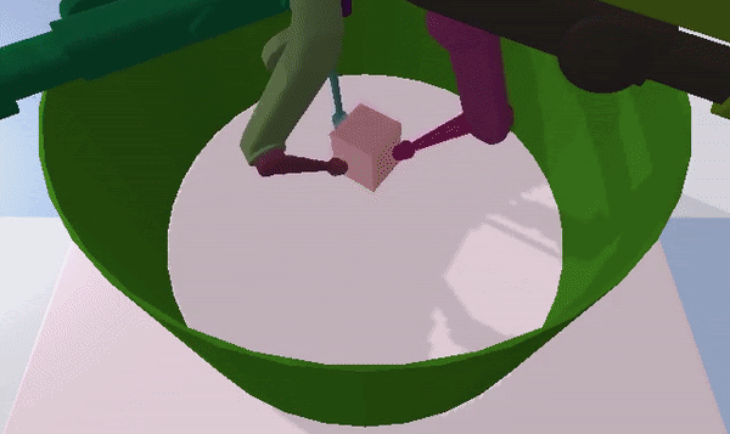
\includegraphics[width=0.9\linewidth]{images/visual_control_envs/causal_world.png}
%     \end{subfigure}
%     \begin{subfigure}{.49\textwidth}
%         \centering
%             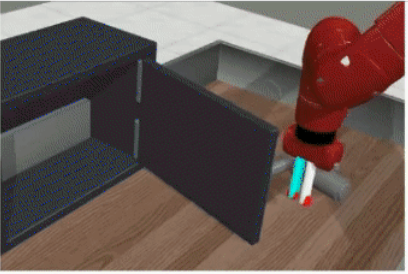
\includegraphics[width=0.9\linewidth]{images/visual_control_envs/metaworld.png}
%     \end{subfigure}
%     \end{figure}
% \end{minipage}
% \hfill
% \begin{minipage}[t]{0.48\linewidth}
%     \begin{figure}
%     \begin{subfigure}{.49\textwidth}
%         \centering
%           \includegraphics[width=0.9\linewidth]{images/env/masked_obj.png}
%     \end{subfigure}
%     \begin{subfigure}{.49\textwidth}
%         \centering
%           \includegraphics[width=0.9\linewidth]{images/env/masked_robot.png}
%     \end{subfigure}
%     \end{figure}
    
%     We can introduce structure:
%     \begin{itemize}
%         \item Each observation contains two entities of interest
%         \item Each entity have its own dynamics
%         \item Actor can directly affect or have a long-term influence over object
%     \end{itemize}
% \end{minipage}
\end{frame}

\note{
Many visual control tasks have the following features: there is a single directly controlled by actions manipulator, there is a number of objects, which can not be controlled by agent directly, and successful completion of task involves some type of interaction between actor and object, for example, opening the fridge. We introduce the object-oriented structure to World Model by factoring it.
}
\begin{frame}
\frametitle{Базовая модель: Dreamer}
\begin{columns}
\begin{column}{0.7\textwidth}
% \begin{framefont}{}
\begin{itemize}
    \item Dreamer\footnotemark[1] представляет собой вариационный автоэнкодер (VAE), кодирующий наблюдения и награды  
    \item Он состоит из
    \begin{itemize}
        \item модели репрезентации (энкодера) $q(s_t\mid s_{t-1}, a_{t-1}, o_{t})$
        \item модель среды $p(s_t \mid s_{t-1}, a_{t-1})$
        \item модель наблюдений (декодер изображений) $p(o_t\mid s_t)$
        \item модели награды (декодер наград) $p(r_t\mid s_t)$
    \end{itemize}
    \item Наблюдения $o_{1:T}$ считаются не марковскими, в связи с чем  VAE выводит марковские состояния $s_t$
    \item Стратегия и критик тренируются на траекториях, полученных в "воображении" модели, полученных при помощи модели среды $p(s_t\mid s_{t-1}, a_{t-1})$
\end{itemize}
% \end{framefont}
\end{column}
\begin{column}{0.4\textwidth}

\begin{figure}
\centering
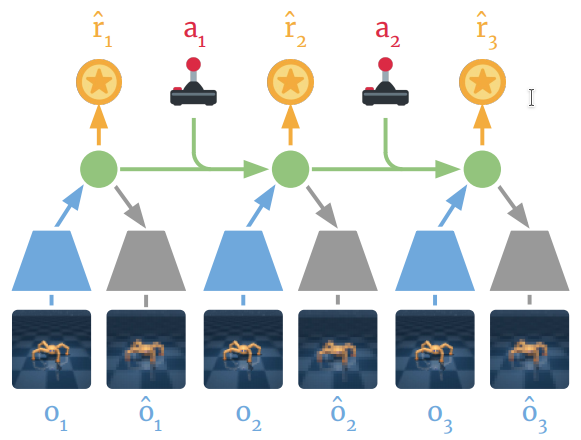
\includegraphics[width=\linewidth]{images/dreamer/1.png}\\
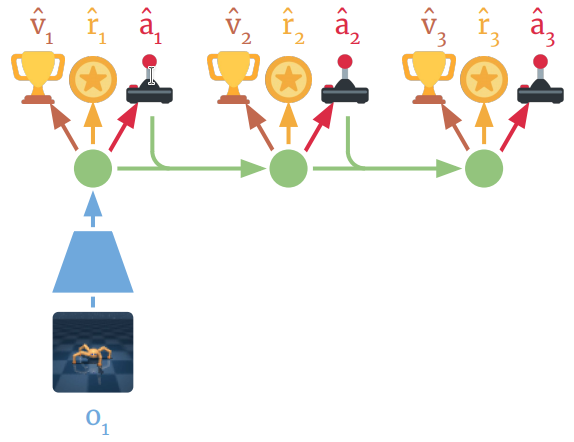
\includegraphics[width=\linewidth]{images/dreamer/2.png}
% \caption{Графическая модель RSSM}
% \label{figM:2}
\end{figure}
\end{column}
\end{columns}
\footnotetext[1]{Danijar Hafner et al. “Dream to Control: Learning Behaviors by Latent Imagination”. In:
ICLR 2020}
\end{frame}
% \input{slides/related_work}
\begin{frame}
\frametitle{Модель мира CEMA}
% TODO: titles are hanging out of images
% TODO: maybe draw commentaries
% TODO: draw an arrow

\begin{columns}[b]
\begin{column}{0.48\linewidth}
\only<1-2>{
    Модель мира Dreamer\cite{Dreamer}:
    \vspace{0.45cm}
    
    \footnotesize{
    \begin{itemize}
    \setlength\itemsep{1ex}
    \setlength\topsep{1.5ex}
        \item $s_t \sim p(s_t \mid s_{t-1}, a_{t-1})$ модель динамики среды
        \item $s_t \sim q(s_t \mid s_{t-1}, a_{t-1}, o_t)$ модель вывода
        \item $p(o_t \mid s_t)$ модель изображения
        \item $p(r_t \mid s_t)$ модель награды
    \end{itemize} }
    \vspace{0.4cm}
    
    \begin{figure}
        \resizebox{.9\linewidth}{!}{\begin{tikzpicture}[scale=2.1]
    \begin{scope}[yshift=8cm,node distance=5em and 5em]
	\path [draw, fill={rgb:red,1;white,3}, rounded corners] (-2.2,-1.5) rectangle (2.0,1.5) {};
	\node[] (rob_dyn) at (-1.0,-1.3) {\LARGE Динамика среды};
    \node[mystyle, fill={rgb:white,1},            ] (st) {\LARGE $s_t$};
    \node[mystyle, fill={rgb:white,1}, left=of st] (stm1) {\LARGE $s_{t-1}$};
    \node[right=of st] (stp1) {};
    \node[mystyle, fill={rgb:white,1}, above left=4em and 3em of st] (atm1) {\LARGE $a_{t-1}$};
    \node[mystyle, fill={rgb:black,1;white,3}, above right=4em and 3em of st] (ot) {\LARGE $o_t$};
    \node[mystyle, fill={rgb:black,1;white,3}, below right=4em and 3em of st] (rt) {\LARGE $r_t$};
    
    \draw[myline] (stm1) -- (st);
	\draw[myline] (atm1) -- (st);
	\draw[myline] (st) -- (ot);
	\draw[myline] (st) -- (rt);
	\draw[myline] (st) -- (stp1);
	
	\draw[myline, dashed, color={rgb:red,2;black,1}] (stm1) edge[bend left] (st);
	\draw[myline, dashed, color={rgb:red,2;black,1}] (ot) edge[bend left] (st);
	\end{scope}
\end{tikzpicture}}
    \end{figure}
}
\only<3->{
    Части модели мира:
    
    \vspace{0.5cm}
    \footnotesize{\textbf{Генеративная} модель прямой причинности:}
    \scriptsize{
    \begin{itemize}
    \setlength\itemsep{1ex}
    \setlength\topsep{1.5ex}
        \item<3-> $s_t \sim p(s_t \mid s_{t-1}, a_{t-1})$ модель динамики скрытых состояний
        \item<4-> $u_t \sim p(u_t \mid s_t, c)$ модель прямой причинности
        \item<5-> $s'_t \sim p(s'_t\mid s'_{t-1}, u_t)$ модель обновления 
    \end{itemize} }
    \vspace{0.4cm}
    \footnotesize{Обратная причинная модель (\textbf{модель вывода})}:
    \scriptsize{
    \begin{itemize}
    \setlength\itemsep{1ex}
    \setlength\topsep{1.5ex}
        \item<3-> $s_t \sim q(s_t \mid s_{t-1}, a_{t-1}, o_t)$ модель вывода состояния робота 
        \item<8-> $s'_t \sim q(s'_t \mid o'_t)$ модель вывода объектного состояния
        \item<9-> $u_t \sim q(u_t \mid s_t, s'_t)$ модель обратной причинности
    \end{itemize} }
    \vspace{0.4cm}
    \footnotesize{Выходы нейронной сети}:
    \scriptsize{
    \begin{itemize}
    \setlength\itemsep{1ex}
    \setlength\topsep{1.5ex}
        \item<3-> $p(o_t \mid s_t)$ субъектный декодер 
        \item<5-> $p(o'_t \mid s'_t)$ объектный декодер
        \item<6-> $p(r_t \mid u_t)$ декодер награды
        \item<10->$\pi(a_t \mid s_t, c)$, $v(s_{t}, u_{t}, s'_{t})$ стратегия и функция полезности
    \end{itemize} }
    \vspace{0.1cm}
}
\end{column}

\begin{column}{0.48\linewidth}
\only<2-10>{
    Модель мира CEMA:
    \begin{figure}
        \resizebox{.9\linewidth}{!}{\begin{frame}
\frametitle{Модель мира CEMA}
% TODO: titles are hanging out of images
% TODO: maybe draw commentaries
% TODO: draw an arrow

\begin{columns}[b]
\begin{column}{0.48\linewidth}
\only<1-2>{
    Модель мира Dreamer\cite{Dreamer}:
    \vspace{0.45cm}
    
    \footnotesize{
    \begin{itemize}
    \setlength\itemsep{1ex}
    \setlength\topsep{1.5ex}
        \item $s_t \sim p(s_t \mid s_{t-1}, a_{t-1})$ модель динамики среды
        \item $s_t \sim q(s_t \mid s_{t-1}, a_{t-1}, o_t)$ модель вывода
        \item $p(o_t \mid s_t)$ модель изображения
        \item $p(r_t \mid s_t)$ модель награды
    \end{itemize} }
    \vspace{0.4cm}
    
    \begin{figure}
        \resizebox{.9\linewidth}{!}{\begin{tikzpicture}[scale=2.1]
    \begin{scope}[yshift=8cm,node distance=5em and 5em]
	\path [draw, fill={rgb:red,1;white,3}, rounded corners] (-2.2,-1.5) rectangle (2.0,1.5) {};
	\node[] (rob_dyn) at (-1.0,-1.3) {\LARGE Динамика среды};
    \node[mystyle, fill={rgb:white,1},            ] (st) {\LARGE $s_t$};
    \node[mystyle, fill={rgb:white,1}, left=of st] (stm1) {\LARGE $s_{t-1}$};
    \node[right=of st] (stp1) {};
    \node[mystyle, fill={rgb:white,1}, above left=4em and 3em of st] (atm1) {\LARGE $a_{t-1}$};
    \node[mystyle, fill={rgb:black,1;white,3}, above right=4em and 3em of st] (ot) {\LARGE $o_t$};
    \node[mystyle, fill={rgb:black,1;white,3}, below right=4em and 3em of st] (rt) {\LARGE $r_t$};
    
    \draw[myline] (stm1) -- (st);
	\draw[myline] (atm1) -- (st);
	\draw[myline] (st) -- (ot);
	\draw[myline] (st) -- (rt);
	\draw[myline] (st) -- (stp1);
	
	\draw[myline, dashed, color={rgb:red,2;black,1}] (stm1) edge[bend left] (st);
	\draw[myline, dashed, color={rgb:red,2;black,1}] (ot) edge[bend left] (st);
	\end{scope}
\end{tikzpicture}}
    \end{figure}
}
\only<3->{
    Части модели мира:
    
    \vspace{0.5cm}
    \footnotesize{\textbf{Генеративная} модель прямой причинности:}
    \scriptsize{
    \begin{itemize}
    \setlength\itemsep{1ex}
    \setlength\topsep{1.5ex}
        \item<3-> $s_t \sim p(s_t \mid s_{t-1}, a_{t-1})$ модель динамики скрытых состояний
        \item<4-> $u_t \sim p(u_t \mid s_t, c)$ модель прямой причинности
        \item<5-> $s'_t \sim p(s'_t\mid s'_{t-1}, u_t)$ модель обновления 
    \end{itemize} }
    \vspace{0.4cm}
    \footnotesize{Обратная причинная модель (\textbf{модель вывода})}:
    \scriptsize{
    \begin{itemize}
    \setlength\itemsep{1ex}
    \setlength\topsep{1.5ex}
        \item<3-> $s_t \sim q(s_t \mid s_{t-1}, a_{t-1}, o_t)$ модель вывода состояния робота 
        \item<8-> $s'_t \sim q(s'_t \mid o'_t)$ модель вывода объектного состояния
        \item<9-> $u_t \sim q(u_t \mid s_t, s'_t)$ модель обратной причинности
    \end{itemize} }
    \vspace{0.4cm}
    \footnotesize{Выходы нейронной сети}:
    \scriptsize{
    \begin{itemize}
    \setlength\itemsep{1ex}
    \setlength\topsep{1.5ex}
        \item<3-> $p(o_t \mid s_t)$ субъектный декодер 
        \item<5-> $p(o'_t \mid s'_t)$ объектный декодер
        \item<6-> $p(r_t \mid u_t)$ декодер награды
        \item<10->$\pi(a_t \mid s_t, c)$, $v(s_{t}, u_{t}, s'_{t})$ стратегия и функция полезности
    \end{itemize} }
    \vspace{0.1cm}
}
\end{column}

\begin{column}{0.48\linewidth}
\only<2-10>{
    Модель мира CEMA:
    \begin{figure}
        \resizebox{.9\linewidth}{!}{\begin{frame}
\frametitle{Модель мира CEMA}
% TODO: titles are hanging out of images
% TODO: maybe draw commentaries
% TODO: draw an arrow

\begin{columns}[b]
\begin{column}{0.48\linewidth}
\only<1-2>{
    Модель мира Dreamer\cite{Dreamer}:
    \vspace{0.45cm}
    
    \footnotesize{
    \begin{itemize}
    \setlength\itemsep{1ex}
    \setlength\topsep{1.5ex}
        \item $s_t \sim p(s_t \mid s_{t-1}, a_{t-1})$ модель динамики среды
        \item $s_t \sim q(s_t \mid s_{t-1}, a_{t-1}, o_t)$ модель вывода
        \item $p(o_t \mid s_t)$ модель изображения
        \item $p(r_t \mid s_t)$ модель награды
    \end{itemize} }
    \vspace{0.4cm}
    
    \begin{figure}
        \resizebox{.9\linewidth}{!}{\input{images/schemes/dreamer_wm}}
    \end{figure}
}
\only<3->{
    Части модели мира:
    
    \vspace{0.5cm}
    \footnotesize{\textbf{Генеративная} модель прямой причинности:}
    \scriptsize{
    \begin{itemize}
    \setlength\itemsep{1ex}
    \setlength\topsep{1.5ex}
        \item<3-> $s_t \sim p(s_t \mid s_{t-1}, a_{t-1})$ модель динамики скрытых состояний
        \item<4-> $u_t \sim p(u_t \mid s_t, c)$ модель прямой причинности
        \item<5-> $s'_t \sim p(s'_t\mid s'_{t-1}, u_t)$ модель обновления 
    \end{itemize} }
    \vspace{0.4cm}
    \footnotesize{Обратная причинная модель (\textbf{модель вывода})}:
    \scriptsize{
    \begin{itemize}
    \setlength\itemsep{1ex}
    \setlength\topsep{1.5ex}
        \item<3-> $s_t \sim q(s_t \mid s_{t-1}, a_{t-1}, o_t)$ модель вывода состояния робота 
        \item<8-> $s'_t \sim q(s'_t \mid o'_t)$ модель вывода объектного состояния
        \item<9-> $u_t \sim q(u_t \mid s_t, s'_t)$ модель обратной причинности
    \end{itemize} }
    \vspace{0.4cm}
    \footnotesize{Выходы нейронной сети}:
    \scriptsize{
    \begin{itemize}
    \setlength\itemsep{1ex}
    \setlength\topsep{1.5ex}
        \item<3-> $p(o_t \mid s_t)$ субъектный декодер 
        \item<5-> $p(o'_t \mid s'_t)$ объектный декодер
        \item<6-> $p(r_t \mid u_t)$ декодер награды
        \item<10->$\pi(a_t \mid s_t, c)$, $v(s_{t}, u_{t}, s'_{t})$ стратегия и функция полезности
    \end{itemize} }
    \vspace{0.1cm}
}
\end{column}

\begin{column}{0.48\linewidth}
\only<2-10>{
    Модель мира CEMA:
    \begin{figure}
        \resizebox{.9\linewidth}{!}{\input{images/schemes/cema_wm}}
    \end{figure}
}
\end{column}
\end{columns}

\note[item]<1->{Let's take a look at RSSM World Model used in Dreamer. It has a single dynamics model and a single latent state, representing the state of the whole environment.}
\note[item]<2->{In CEMA, we split dynamics model on two parts: robot dynamics and object dynamics.}
\note[item]<3->{For robot dynamics, we left the RSSM without any changes, since the robot state is controlled directly by actions.}
\note[item]<4->{From imagined robot latent state, we predict the task-specific influence vector, which represents the collateral object control performed by robot.}
\note[item]<5->{The next object state is predicted using RSSM and the imagined influence vector.}
\note[item]<6->{The influence vector is also used to predict step reward.}
\note[item]<7->{The inference model of actor remains unchanged to Dreamer, specifically, the robot state is inferred from its previous state and current robot observation.}
\note[item]<8->{Object latent state, on contrary, is inferred from the object image alone.}
\note[item]<9->{For influence vector, posterior distribution is conditioned on both object and actor latent states to reflect the changes made to object by actor.}
\note[item]<10->{Value function is conditioned on all latent states, while policy is conditioned only on robot state and low-dimensional task context vector.}
\end{frame}}
    \end{figure}
}
\end{column}
\end{columns}

\note[item]<1->{Let's take a look at RSSM World Model used in Dreamer. It has a single dynamics model and a single latent state, representing the state of the whole environment.}
\note[item]<2->{In CEMA, we split dynamics model on two parts: robot dynamics and object dynamics.}
\note[item]<3->{For robot dynamics, we left the RSSM without any changes, since the robot state is controlled directly by actions.}
\note[item]<4->{From imagined robot latent state, we predict the task-specific influence vector, which represents the collateral object control performed by robot.}
\note[item]<5->{The next object state is predicted using RSSM and the imagined influence vector.}
\note[item]<6->{The influence vector is also used to predict step reward.}
\note[item]<7->{The inference model of actor remains unchanged to Dreamer, specifically, the robot state is inferred from its previous state and current robot observation.}
\note[item]<8->{Object latent state, on contrary, is inferred from the object image alone.}
\note[item]<9->{For influence vector, posterior distribution is conditioned on both object and actor latent states to reflect the changes made to object by actor.}
\note[item]<10->{Value function is conditioned on all latent states, while policy is conditioned only on robot state and low-dimensional task context vector.}
\end{frame}}
    \end{figure}
}
\end{column}
\end{columns}

\note[item]<1->{Let's take a look at RSSM World Model used in Dreamer. It has a single dynamics model and a single latent state, representing the state of the whole environment.}
\note[item]<2->{In CEMA, we split dynamics model on two parts: robot dynamics and object dynamics.}
\note[item]<3->{For robot dynamics, we left the RSSM without any changes, since the robot state is controlled directly by actions.}
\note[item]<4->{From imagined robot latent state, we predict the task-specific influence vector, which represents the collateral object control performed by robot.}
\note[item]<5->{The next object state is predicted using RSSM and the imagined influence vector.}
\note[item]<6->{The influence vector is also used to predict step reward.}
\note[item]<7->{The inference model of actor remains unchanged to Dreamer, specifically, the robot state is inferred from its previous state and current robot observation.}
\note[item]<8->{Object latent state, on contrary, is inferred from the object image alone.}
\note[item]<9->{For influence vector, posterior distribution is conditioned on both object and actor latent states to reflect the changes made to object by actor.}
\note[item]<10->{Value function is conditioned on all latent states, while policy is conditioned only on robot state and low-dimensional task context vector.}
\end{frame}
% \begin{frame}
\frametitle{Вариации структуры}
% \begin{framefont}{}
\begin{figure}[ht]%{r}{0.35\textwidth}
    % \centering
    % \vspace{-80pt}
    \scalebox{0.7}{
        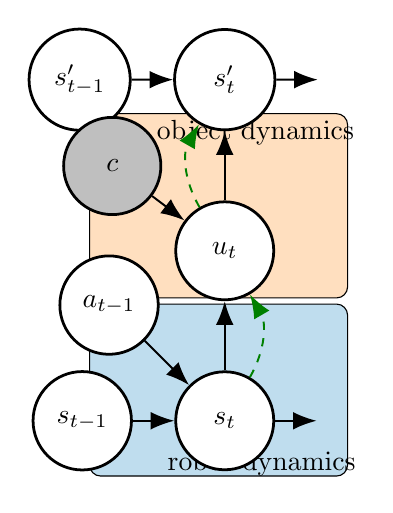
\begin{tikzpicture}[scale=0.78]
    \begin{scope}[yshift=8cm,node distance=2.5em and 1.5em]
	\path [draw, fill={rgb:blue,1;white,3}, rounded corners] (-2.2,-0.9) rectangle (2.0,1.9) {};
	\path [draw, fill={rgb:orange,1;white,3}, rounded corners] (-2.2,2.0) rectangle (2.0,5.0) {};
	\node[] (rob_dyn) at (0.6,-0.7) {robot dynamics};
	\node[] (obj_dyn) at (0.5,4.7) {object dynamics};
    \node[mystyle, fill={rgb:white,1},            ] (st) {$s_t$};
    \node[mystyle, fill={rgb:white,1}, above=of st] (ut) {$u_t$};
    \node[mystyle, fill={rgb:white,1}, above=of ut] (sts) {$s'_t$};
    \node[mystyle, fill={rgb:white,1}, left=of sts] (stsm1) {$s'_{t-1}$};
    \node[right=of sts] (stsp1) {};
    % \node[mystyle, fill={rgb:black,1;white,3}, below right=1.6em and 1.6em of sts] (ots) {$o'_t$};
    % \node[mystyle, fill={rgb:black,1;white,3}, above left=1.2em and 0.0em of ut] (rt) {$r_t$};
    \node[mystyle, fill={rgb:black,1;white,3}, above left=0.5em and 1.5em of ut] (c) {$c$};
    \node[mystyle, fill={rgb:white,1}, left=of st] (stm1) {$s_{t-1}$};
    \node[mystyle, fill={rgb:white,1}, above left=1.6em and 1.6em of st] (atm1) {$a_{t-1}$};
    % \node[mystyle, fill={rgb:black,1;white,3}, above right=1.6em and 1.6em of st] (ot) {$o_t$};
    % \node[mystyle, fill={rgb:black,1;brown,3}, above left=0.9em and 0.1em of ut] (u1t) {$u_t$};
    \node[right=of st] (stp1) {};
    \draw[myline] (stsm1) -- (sts);
	\draw[myline] (sts) -- (stsp1);
% 	\draw[myline] (sts) -- (ots);
	\draw[myline] (st) -- (ut);
	\draw[myline] (ut) -- (sts);
	\draw[myline] (stm1) -- (st);
	\draw[myline] (atm1) -- (st);
% 	\draw[myline] (st) -- (ot);
	\draw[myline] (c) -- (ut);
% 	\draw[myline] (ut) -- (rt);
	\draw[myline] (st) -- (stp1);
% 	\draw[myline, dashed, color=blue] (ots) edge[bend right] (sts);
% 	\draw[myline, color={rgb:brown,1;black,1}] (ots) edge[bend right=20, mysnake,] (ut);
% 	\draw[myline, color={rgb:brown,1;black,1}] (st) edge[bend left=20, mysnake,] (ut);
	\draw[myline, dashed, color={rgb:green,1;black,1}] (ut) edge[bend left] (sts);
	\draw[myline, dashed, color={rgb:green,1;black,1}] (st) edge[bend right] (ut);
	
% 	\draw[myline, dashed, color={rgb:red,2;black,1}] (stm1) edge[bend left] (st);
% 	\draw[myline, dashed, color={rgb:red,2;black,1}] (atm1) edge[bend left] (st);
% 	\draw[myline, dashed, color={rgb:red,2;black,1}] (ot) edge[bend left] (st);
	\end{scope}
  \end{tikzpicture}
    }
    \scalebox{0.7}{
        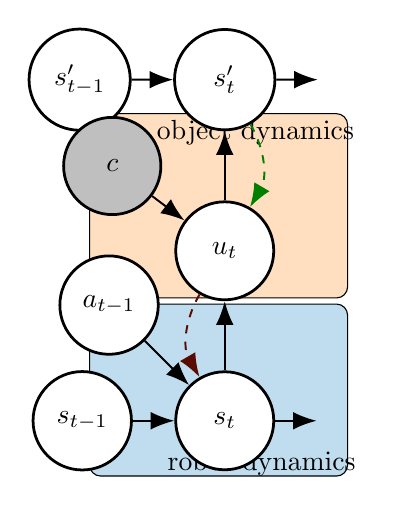
\begin{tikzpicture}[scale=0.78]
    \begin{scope}[yshift=8cm,node distance=2.5em and 1.5em]
	\path [draw, fill={rgb:blue,1;white,3}, rounded corners] (-2.2,-0.9) rectangle (2.0,1.9) {};
	\path [draw, fill={rgb:orange,1;white,3}, rounded corners] (-2.2,2.0) rectangle (2.0,5.0) {};
	\node[] (rob_dyn) at (0.6,-0.7) {robot dynamics};
	\node[] (obj_dyn) at (0.5,4.7) {object dynamics};
    \node[mystyle, fill={rgb:white,1},            ] (st) {$s_t$};
    \node[mystyle, fill={rgb:white,1}, above=of st] (ut) {$u_t$};
    \node[mystyle, fill={rgb:white,1}, above=of ut] (sts) {$s'_t$};
    \node[mystyle, fill={rgb:white,1}, left=of sts] (stsm1) {$s'_{t-1}$};
    \node[right=of sts] (stsp1) {};
    % \node[mystyle, fill={rgb:black,1;white,3}, below right=1.6em and 1.6em of sts] (ots) {$o'_t$};
    % \node[mystyle, fill={rgb:black,1;white,3}, above left=1.2em and 0.0em of ut] (rt) {$r_t$};
    \node[mystyle, fill={rgb:black,1;white,3}, above left=0.5em and 1.5em of ut] (c) {$c$};
    \node[mystyle, fill={rgb:white,1}, left=of st] (stm1) {$s_{t-1}$};
    \node[mystyle, fill={rgb:white,1}, above left=1.6em and 1.6em of st] (atm1) {$a_{t-1}$};
    % \node[mystyle, fill={rgb:black,1;white,3}, above right=1.6em and 1.6em of st] (ot) {$o_t$};
    % \node[mystyle, fill={rgb:black,1;brown,3}, above left=0.9em and 0.1em of ut] (u1t) {$u_t$};
    \node[right=of st] (stp1) {};
    \draw[myline] (stsm1) -- (sts);
	\draw[myline] (sts) -- (stsp1);
% 	\draw[myline] (sts) -- (ots);
	\draw[myline] (st) -- (ut);
	\draw[myline] (ut) -- (sts);
	\draw[myline] (stm1) -- (st);
	\draw[myline] (atm1) -- (st);
% 	\draw[myline] (st) -- (ot);
	\draw[myline] (c) -- (ut);
% 	\draw[myline] (ut) -- (rt);
	\draw[myline] (st) -- (stp1);
% 	\draw[myline, dashed, color=blue] (ots) edge[bend right] (sts);
% 	\draw[myline, color={rgb:brown,1;black,1}] (ots) edge[bend right=20, mysnake,] (ut);
% 	\draw[myline, color={rgb:brown,1;black,1}] (st) edge[bend left=20, mysnake,] (ut);
	\draw[myline, dashed, color={rgb:green,1;black,1}] (sts) edge[bend left] (ut);
	\draw[myline, dashed, color={rgb:red,1;black,1}] (ut) edge[bend right] (st);
	
% 	\draw[myline, dashed, color={rgb:red,2;black,1}] (stm1) edge[bend left] (st);
% 	\draw[myline, dashed, color={rgb:red,2;black,1}] (atm1) edge[bend left] (st);
% 	\draw[myline, dashed, color={rgb:red,2;black,1}] (ot) edge[bend left] (st);
	\end{scope}
  \end{tikzpicture}
    }
    \scalebox{0.7}{
        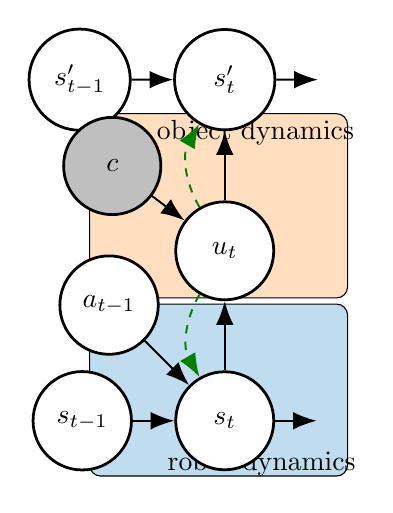
\begin{tikzpicture}[scale=0.78]
    \begin{scope}[yshift=8cm,node distance=2.5em and 1.5em]
	\path [draw, fill={rgb:blue,1;white,3}, rounded corners] (-2.2,-0.9) rectangle (2.0,1.9) {};
	\path [draw, fill={rgb:orange,1;white,3}, rounded corners] (-2.2,2.0) rectangle (2.0,5.0) {};
	\node[] (rob_dyn) at (0.6,-0.7) {robot dynamics};
	\node[] (obj_dyn) at (0.5,4.7) {object dynamics};
    \node[mystyle, fill={rgb:white,1},            ] (st) {$s_t$};
    \node[mystyle, fill={rgb:white,1}, above=of st] (ut) {$u_t$};
    \node[mystyle, fill={rgb:white,1}, above=of ut] (sts) {$s'_t$};
    \node[mystyle, fill={rgb:white,1}, left=of sts] (stsm1) {$s'_{t-1}$};
    \node[right=of sts] (stsp1) {};
    % \node[mystyle, fill={rgb:black,1;white,3}, below right=1.6em and 1.6em of sts] (ots) {$o'_t$};
    % \node[mystyle, fill={rgb:black,1;white,3}, above left=1.2em and 0.0em of ut] (rt) {$r_t$};
    \node[mystyle, fill={rgb:black,1;white,3}, above left=0.5em and 1.5em of ut] (c) {$c$};
    \node[mystyle, fill={rgb:white,1}, left=of st] (stm1) {$s_{t-1}$};
    \node[mystyle, fill={rgb:white,1}, above left=1.6em and 1.6em of st] (atm1) {$a_{t-1}$};
    % \node[mystyle, fill={rgb:black,1;white,3}, above right=1.6em and 1.6em of st] (ot) {$o_t$};
    % \node[mystyle, fill={rgb:black,1;brown,3}, above left=0.9em and 0.1em of ut] (u1t) {$u_t$};
    \node[right=of st] (stp1) {};
    \draw[myline] (stsm1) -- (sts);
	\draw[myline] (sts) -- (stsp1);
% 	\draw[myline] (sts) -- (ots);
	\draw[myline] (st) -- (ut);
	\draw[myline] (ut) -- (sts);
	\draw[myline] (stm1) -- (st);
	\draw[myline] (atm1) -- (st);
% 	\draw[myline] (st) -- (ot);
	\draw[myline] (c) -- (ut);
% 	\draw[myline] (ut) -- (rt);
	\draw[myline] (st) -- (stp1);
% 	\draw[myline, dashed, color=blue] (ots) edge[bend right] (sts);
% 	\draw[myline, color={rgb:brown,1;black,1}] (ots) edge[bend right=20, mysnake,] (ut);
% 	\draw[myline, color={rgb:brown,1;black,1}] (st) edge[bend left=20, mysnake,] (ut);
	\draw[myline, dashed, color={rgb:green,1;black,1}] (ut) edge[bend left] (sts);
	\draw[myline, dashed, color={rgb:green,1;black,1}] (ut) edge[bend right] (st);
	
% 	\draw[myline, dashed, color={rgb:red,2;black,1}] (stm1) edge[bend left] (st);
% 	\draw[myline, dashed, color={rgb:red,2;black,1}] (atm1) edge[bend left] (st);
% 	\draw[myline, dashed, color={rgb:red,2;black,1}] (ot) edge[bend left] (st);
	\end{scope}
  \end{tikzpicture}
    }
    \scalebox{0.7}{
        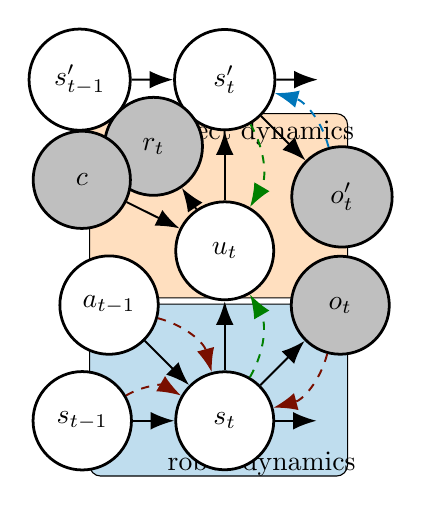
\begin{tikzpicture}[scale=0.78]
    \begin{scope}[yshift=8cm,node distance=2.5em and 1.5em]
	\path [draw, fill={rgb:blue,1;white,3}, rounded corners] (-2.2,-0.9) rectangle (2.0,1.9) {};
	\path [draw, fill={rgb:orange,1;white,3}, rounded corners] (-2.2,2.0) rectangle (2.0,5.0) {};
	\node[] (rob_dyn) at (0.6,-0.7) {robot dynamics};
	\node[] (obj_dyn) at (0.5,4.7) {object dynamics};
    \node[mystyle, fill={rgb:white,1},            ] (st) {$s_t$};
    \node[mystyle, fill={rgb:white,1}, above=of st] (ut) {$u_t$};
    \node[mystyle, fill={rgb:white,1}, above=of ut] (sts) {$s'_t$};
    \node[mystyle, fill={rgb:white,1}, left=of sts] (stsm1) {$s'_{t-1}$};
    \node[right=of sts] (stsp1) {};
    \node[mystyle, fill={rgb:black,1;white,3}, below right=1.6em and 1.6em of sts] (ots) {$o'_t$};
    \node[mystyle, fill={rgb:black,1;white,3}, above left=1.2em and 0.0em of ut] (rt) {$r_t$};
    \node[mystyle, fill={rgb:black,1;white,3}, above left=0.0em and 2.6em of ut] (c) {$c$};
    \node[mystyle, fill={rgb:white,1}, left=of st] (stm1) {$s_{t-1}$};
    \node[mystyle, fill={rgb:white,1}, above left=1.6em and 1.6em of st] (atm1) {$a_{t-1}$};
    \node[mystyle, fill={rgb:black,1;white,3}, above right=1.6em and 1.6em of st] (ot) {$o_t$};
    % \node[mystyle, fill={rgb:black,1;brown,3}, above left=0.9em and 0.1em of ut] (u1t) {$u_t$};
    \node[right=of st] (stp1) {};
    \draw[myline] (stsm1) -- (sts);
	\draw[myline] (sts) -- (stsp1);
	\draw[myline] (sts) -- (ots);
	\draw[myline] (st) -- (ut);
	\draw[myline] (ut) -- (sts);
	\draw[myline] (stm1) -- (st);
	\draw[myline] (atm1) -- (st);
	\draw[myline] (st) -- (ot);
	\draw[myline] (c) -- (ut);
	\draw[myline] (ut) -- (rt);
	\draw[myline] (st) -- (stp1);
	\draw[myline, dashed, color=blue] (ots) edge[bend right] (sts);
% 	\draw[myline, color={rgb:brown,1;black,1}] (ots) edge[bend right=20, mysnake,] (ut);
% 	\draw[myline, color={rgb:brown,1;black,1}] (st) edge[bend left=20, mysnake,] (ut);
	\draw[myline, dashed, color={rgb:green,1;black,1}] (sts) edge[bend left] (ut);
	\draw[myline, dashed, color={rgb:green,1;black,1}] (st) edge[bend right] (ut);
	
	\draw[myline, dashed, color={rgb:red,2;black,1}] (stm1) edge[bend left] (st);
	\draw[myline, dashed, color={rgb:red,2;black,1}] (atm1) edge[bend left] (st);
	\draw[myline, dashed, color={rgb:red,2;black,1}] (ot) edge[bend left] (st);
	\end{scope}
  \end{tikzpicture}
    }
    % \caption{\textbf{First, Second, Third columns}: Different variations in the inference model related to the influence model. 
    % Graphical model for the factorized agent. Solid lines indicate generative distributions; dashed lines indicate inference distribution. \textbf{Fourth column}: The full CEMA model scheme. Solid lines indicate generative distributions; dashed lines indicate inference distributions. The dashed color indicates the kind of distribution for clarity: red for the robot state inference, green for the influence state inference, and blue for the object state influence.}
    \label{model_variations}
    \vspace{-20pt}
\end{figure}
\end{frame}
\begin{frame}
\frametitle{Тренировочный процесс}

\begin{figure}
    \centering
    \resizebox{.9\linewidth}{!}{\definecolor{myblue}{rgb}{0.29,0.5647,0.8862}
\definecolor{myred}{rgb}{0.8776,0.0084,0.1139}
\definecolor{myyellow}{rgb}{0.9607,0.6509,0.1372}
\definecolor{myygreen}{rgb}{0.4941,0.8274,0.1294}
\tikzset{
  font={\fontsize{14pt}{12}\selectfont}}
  
\tikzset{
state/.style={
  circle,
  line width=3pt,
  text width=2em,
  align=center,
  fill=myygreen,
  draw=white,
  }
}

\tikzset{
trap/.style={
  trapezium,
  trapezium stretches=true, 
  minimum width=1.2cm, 
  trapezium angle=75, 
  minimum height=0.8cm,
  line width=3pt,
  fill={rgb:myblue,},
  draw=white,
  }
}

\tikzset{
imagline/.style={
  line width=3pt,
  }
}
\tikzset{
imagsnake/.style={
  decoration={snake, pre length=0.01mm, segment length=2mm, amplitude=0.3mm, post length=3mm},
  decorate
  }
}

\begin{tikzpicture}
    % middle part
    \node[state, minimum size=1cm, visible on=<2->] (st) {};
    \node[trap, below left=0.6cm and 0.1cm of st, visible on=<2->] (tr1) {};
    \node[trap, below right=0.6cm and 0.1cm of st, visible on=<2->] (tr2) {};
    \node[above left=0.4cm and 0.3cm of st, visible on=<2->] (at) {$a_1$};
    \node[above=0.5cm of st, visible on=<2->] (rt) {$\widehat{r_1}$};
    
    \node[below=-0.15cm of tr1, visible on=<2->] (o1_wm) {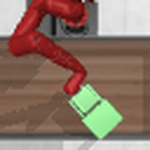
\includegraphics[width=1.1cm]{images/utils/o1_wm_tr.png}};
    \node[below=-0.15cm of tr2, visible on=<2->] (o2_wm) {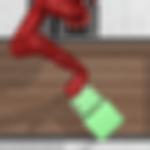
\includegraphics[width=1.1cm]{images/utils/o2_wm_tr.png}};
    \node[below=-0.05cm of o1_wm, visible on=<2->] (o1) {$o_1$};
    \node[below=-0.15cm of o2_wm, visible on=<2->] (o2) {$\widehat{o_1}$};
    
    \node[state, minimum size=1cm, right=1.5cm of st, visible on=<2->] (st1) {};
    \node[above left=0.4cm and 0.3cm of st1, visible on=<2->] (at1) {$a_2$};
    \node[above=0.5cm of st1, visible on=<2->] (rt1) {$\widehat{r_2}$};
    
    \draw[imagline, color=myblue, visible on=<2->] (st) -- (tr1.north);
    \draw[imagline, color=myblue, visible on=<2->] (st) -- (tr2.north);
    \draw[imagline, color=myred, visible on=<2->] (at) -- (st);
    \draw[imagline, color=myred, visible on=<2->] (at1) -- (st1);
    \draw[imagline, color=myygreen, visible on=<2->] (st) -- (st1);
    
    \draw[imagline, -{Latex[length=3mm]}, color=myyellow, visible on=<2->] (st) -- (rt);
    \draw[imagline, -{Latex[length=3mm]}, color=myyellow, visible on=<2->] (st1) -- (rt1);
    \node[below right=3.2cm and -1.2cm of st, visible on=<2->] (wm) {Тренировка модели мира};
    
    
    % right part
    \node[state, minimum size=1cm, right=8cm of st, visible on=<3->] (st_p) {};
    \node[trap, below left=0.6cm and 0.1cm of st_p, visible on=<3->] (tr1_p) {};
    
    \node[above left=0.4cm and 0.3cm of st_p, visible on=<3->] (at_p) {$a_1$};
    \node[above=0.5cm of st_p, visible on=<3->] (rt_p) {$\widehat{r_1}$};
    
    \node[below=-0.15cm of tr1_p, visible on=<3->] (o1_p) {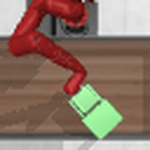
\includegraphics[width=1.1cm, visible on=<4->]{images/utils/o1_wm_tr.png}};
    \node[below=-0.05cm of o1_p, visible on=<3->] (o1_pp) {$o_1$};
    
    \node[state, minimum size=1cm, right=1.5cm of st_p, visible on=<3->] (st1_p) {};
    \node[below left=0.5cm and 0.4cm of st1_p, visible on=<3->] (at1_p) {$a_2$};
    \node[above=0.5cm of st1_p, visible on=<3->] (rt1_p) {$\widehat{r_2}$};
    \node[state, minimum size=1cm, right=1.5cm of st1_p, visible on=<3->] (st2_p) {};
    \node[below left=0.5cm and 0.4cm of st2_p, visible on=<3->] (at2_p) {$a_3$};
    \node[above=0.5cm of st2_p, visible on=<3->] (rt2_p) {$\widehat{r_3}$};
    % densely dotted
    
    \draw[imagline, color=myblue, visible on=<3->] (st_p) -- (tr1_p.north);
    \draw[imagline, color=myred, visible on=<3->] (at_p) -- (st_p);
    \draw[imagline, color=myred, loosely dotted, -{Latex[length=3mm]}, visible on=<3->] (st_p) -- (at1_p);
    \draw[imagline, color=myred, visible on=<3->] (at1_p) -- (st1_p);
    \draw[imagline, color=myygreen, visible on=<3->] (st_p) -- (st1_p);
    
    \draw[imagline, color=myred, loosely dotted, -{Latex[length=3mm]}, visible on=<3->] (st1_p) -- (at2_p);
    \draw[imagline, color=myred, visible on=<3->] (at2_p) -- (st2_p);
    \draw[imagline, color=myygreen, visible on=<3->] (st1_p) -- (st2_p);
    
    
    \draw[imagline, -{Latex[length=3mm]}, color=myyellow, visible on=<3->] (st_p) -- (rt_p);
    \draw[imagline, -{Latex[length=3mm]}, color=myyellow, visible on=<3->] (st1_p) -- (rt1_p);
    \draw[imagline, -{Latex[length=3mm]}, color=myyellow, visible on=<3->] (st2_p) -- (rt2_p);
    \node[below right=3.2cm and -0.2cm of st_p, visible on=<3->] (wm_p) {Тренировка стратегии в ``воображении''};
    
    
    
    % left part
    \node[state, minimum size=1cm, left=9cm of st, visible on=<1->] (st_e) {};
    \node[state, minimum size=1cm, right=1.0cm of st_e, visible on=<1->] (st1_e) {};
    \node[state, minimum size=1cm, right=1.0cm of st1_e, visible on=<1->] (st2_e) {};
    \draw[imagline, color=myygreen, visible on=<1->] (st1_e) -- (st2_e);
    \draw[imagline, color=myygreen, visible on=<1->] (st_e) -- (st1_e);
    
    \node[above left=0.4cm and 0.3cm of st_e, visible on=<1->] (at_e) {$a_1$};
    \draw[imagline, color=myred, visible on=<1->] (at_e) -- (st_e);
    \node[above left=0.4cm and 0.3cm of st1_e, visible on=<1->] (at1_e) {$a_2$};
    \draw[imagline, color=myred, visible on=<1->] (at1_e) -- (st1_e);
    \node[above left=0.4cm and 0.3cm of st2_e, visible on=<1->] (at2_e) {$a_3$};
    \draw[imagline, color=myred, visible on=<1->] (at2_e) -- (st2_e);
    
    
    \node[trap, below left=0.6cm and 0.1cm of st_e, visible on=<1->] (tr1_e) {};
    \draw[imagline, color=myblue, visible on=<1->] (st_e) -- (tr1_e.north);
    \node[below=-0.15cm of tr1_e, visible on=<1->] (o1_e) {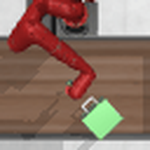
\includegraphics[width=1.1cm]{images/utils/o1_e.png}};
    \node[below=-0.05cm of o1_e, visible on=<1->] (o1_ee) {$o_1$};
    
    \node[trap, below left=0.6cm and 0.1cm of st1_e, visible on=<1->] (tr2_e) {};
    \draw[imagline, color=myblue, visible on=<1->] (st1_e) -- (tr2_e.north);
    \node[below=-0.15cm of tr2_e, visible on=<1->] (o2_e) {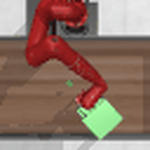
\includegraphics[width=1.1cm]{images/utils/o2_e.png}};
    \node[below=-0.05cm of o2_e, visible on=<1->] (o2_ee) {$o_2$};
    
    \node[trap, below left=0.6cm and 0.1cm of st2_e, visible on=<1->] (tr3_e) {};
    \draw[imagline, color=myblue, visible on=<1->] (st2_e) -- (tr3_e.north);
    \node[below=-0.15cm of tr3_e, visible on=<1->] (o3_e) {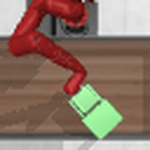
\includegraphics[width=1.1cm]{images/utils/o3_e.png}};
    \node[below=-0.05cm of o3_e, visible on=<1->] (o3_ee) {$o_3$};
    \node[below right=3.2cm and -0.2cm of st_e, visible on=<1->] (wm_e) {Сбор опыта};
    
    
    % black arrows
    \node[right=0.2cm of st2_e, visible on=<2->] (help1l) {};
    \node[left=0.2cm of st, visible on=<2->] (help1r) {};
    \draw[-triangle 45, line width=2mm,
    postaction={draw=black, rounded corners, line width=0.35cm, shorten >=0.5cm, -}, visible on=<2->] (help1l) -- (help1r);
    
    \node[right=0.2cm of st1, visible on=<3->] (help2l) {};
    \node[left=0.2cm of st_p, visible on=<3->] (help2r) {};
    \draw[-triangle 45, line width=2mm,
    postaction={draw=black, rounded corners, line width=0.35cm, shorten >=0.5cm, -}, visible on=<3->] (help2l) -- (help2r);
    
    \node[below=3.8cm of st1_e, visible on=<4->] (help3r) {};
    \node[below=3.8cm of st1_p, visible on=<4->] (help3l) {};
    
    \node[below=1.2cm of help3r, visible on=<4->] (p2) {};
    \node[below=1.2cm of help3l, visible on=<4->] (p1) {};
    \draw[-triangle 45, line width=2mm, rounded corners, 
    postaction={draw=black, line width=0.35cm, shorten >=0.5cm, -}, visible on=<4->] (help3l) -- (p1.north) -- (p2.south) -- (help3r.south);
    
    
\end{tikzpicture}}
\end{figure}
\note[item]<1->{The training process of CEMA is the same as in Dreamer. First, the agent collects experience, interacting with the environment.}
\note[item]<2->{Then, this experience is used to perform self-supervised training of World Model.}
\note[item]<3->{Finally, using the World Model, the actor-critic policy is learned on imagined trajectories.}
\note[item]<4->{The process is repeated and all three steps can be performed in parallel.}
\end{frame}

\begin{frame}
\frametitle{Эксперимент: Rotated Drawer World, описание среды}

\begin{columns}[t]
\begin{column}{0.33\linewidth}<3->
    Пример наблюдения:
    % \begin{itemize}
    %     \item Each observation contains two entities of interest
    %     \item Each entity have its own dynamics
    %     \item Actor can directly affect or have a long-term influence over object
    % \end{itemize}
    \begin{itemize}
        \item<4-> Объектная часть
            \begin{figure}
            \begin{subfigure}{0.8\linewidth}
                \centering
                  \includegraphics[width=\linewidth]{images/env/rotated_drawer/masked_obj.png}
            \end{subfigure}
            \end{figure}
        \item<5-> Субъектная часть
            \begin{figure}
            \begin{subfigure}{0.8\linewidth}
                \centering
                  \includegraphics[width=\linewidth]{images/env/rotated_drawer/masked_robot.png}
            \end{subfigure}
            \end{figure}
    \end{itemize}
\end{column}
\hfill
\begin{column}{0.63\linewidth}<1->
    Среда для эксперимента:
    \begin{figure}
    \onslide<1->{\begin{subfigure}{.4\linewidth}
        \centering
            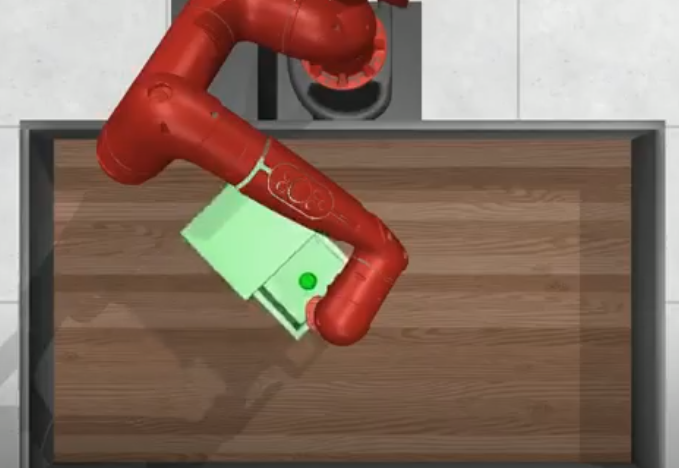
\includegraphics[width=\linewidth]{images/env/rotated_drawer/env_task2.png}
    \end{subfigure}}
    \end{figure}
    \begin{figure}
    \centering
    \onslide<2->{\begin{subfigure}{0.4\linewidth}
        \centering
            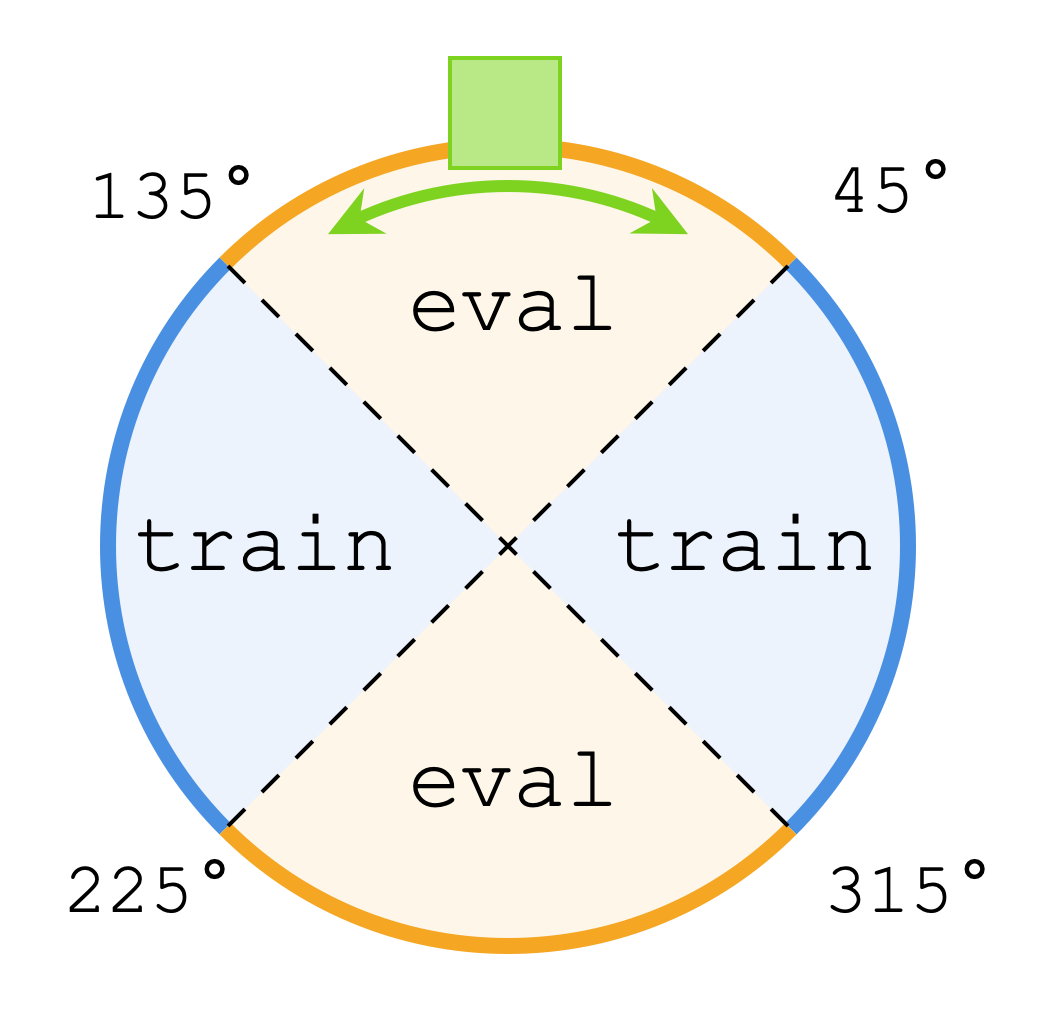
\includegraphics[width=\linewidth]{images/env/rotated_drawer/drawer_tasks.png}
    \end{subfigure}}
    \end{figure}
    \begin{figure}
        \onslide<1->{\begin{subfigure}{.4\linewidth}
            \centering
                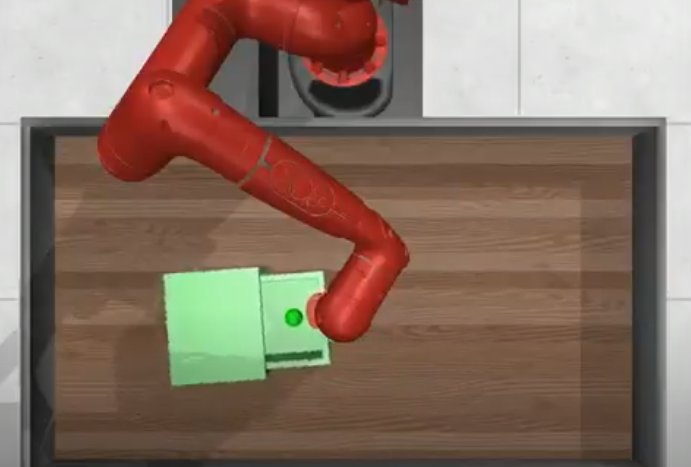
\includegraphics[width=\linewidth]{images/env/rotated_drawer/env_task1.png}
        \end{subfigure}}
        \hspace{3em}%
        \onslide<1->{\begin{subfigure}{.4\linewidth}
            \centering
                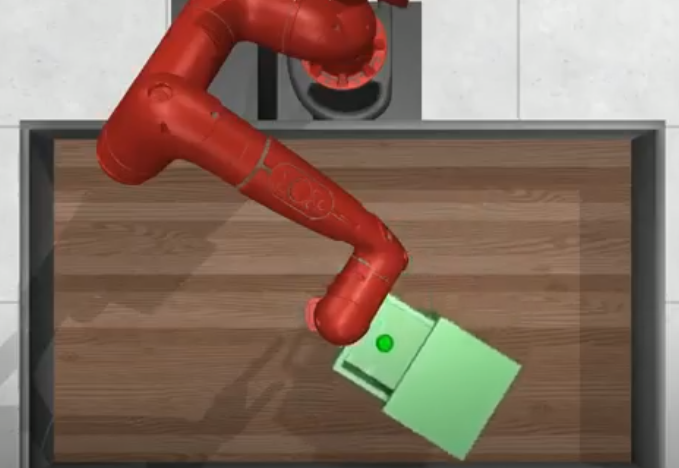
\includegraphics[width=\linewidth]{images/env/rotated_drawer/env_task3.png}
        \end{subfigure}}
    \end{figure}
    
    % Probably not needed
    % \begin{itemize}
    %     \item The task is defined by drawer position
    %     \item Ground truth segmentation masks
    %     \item Out-of-distribution test tasks
    %     \item Single topdown camera for all tasks
    % \end{itemize}
\end{column}
\end{columns}
\note[item]<1->{We built the custom parameterized task environment for evaluating the generalization capabilities of algorithm. It is a drawer, which should be opened by robotic hand.In each specific task, the drawer is fixed.}
\note[item]<2->{The set of tasks then coincides with the set of positions of the drawer, which is a circle with a given radius.}
\note[item]<3->{Each observation consists of two parts:}
\note[item]<4->{the unoccluded object image;}
\note[item]<5->{and the robot image.}
\end{frame}
\begin{frame}
\frametitle{Эксперимент: Rotated Drawer World, результаты}

\begin{columns}[t]
\begin{column}{0.48\linewidth}<1->
    \begin{figure}
        \begin{subfigure}{\linewidth}
        \centering
          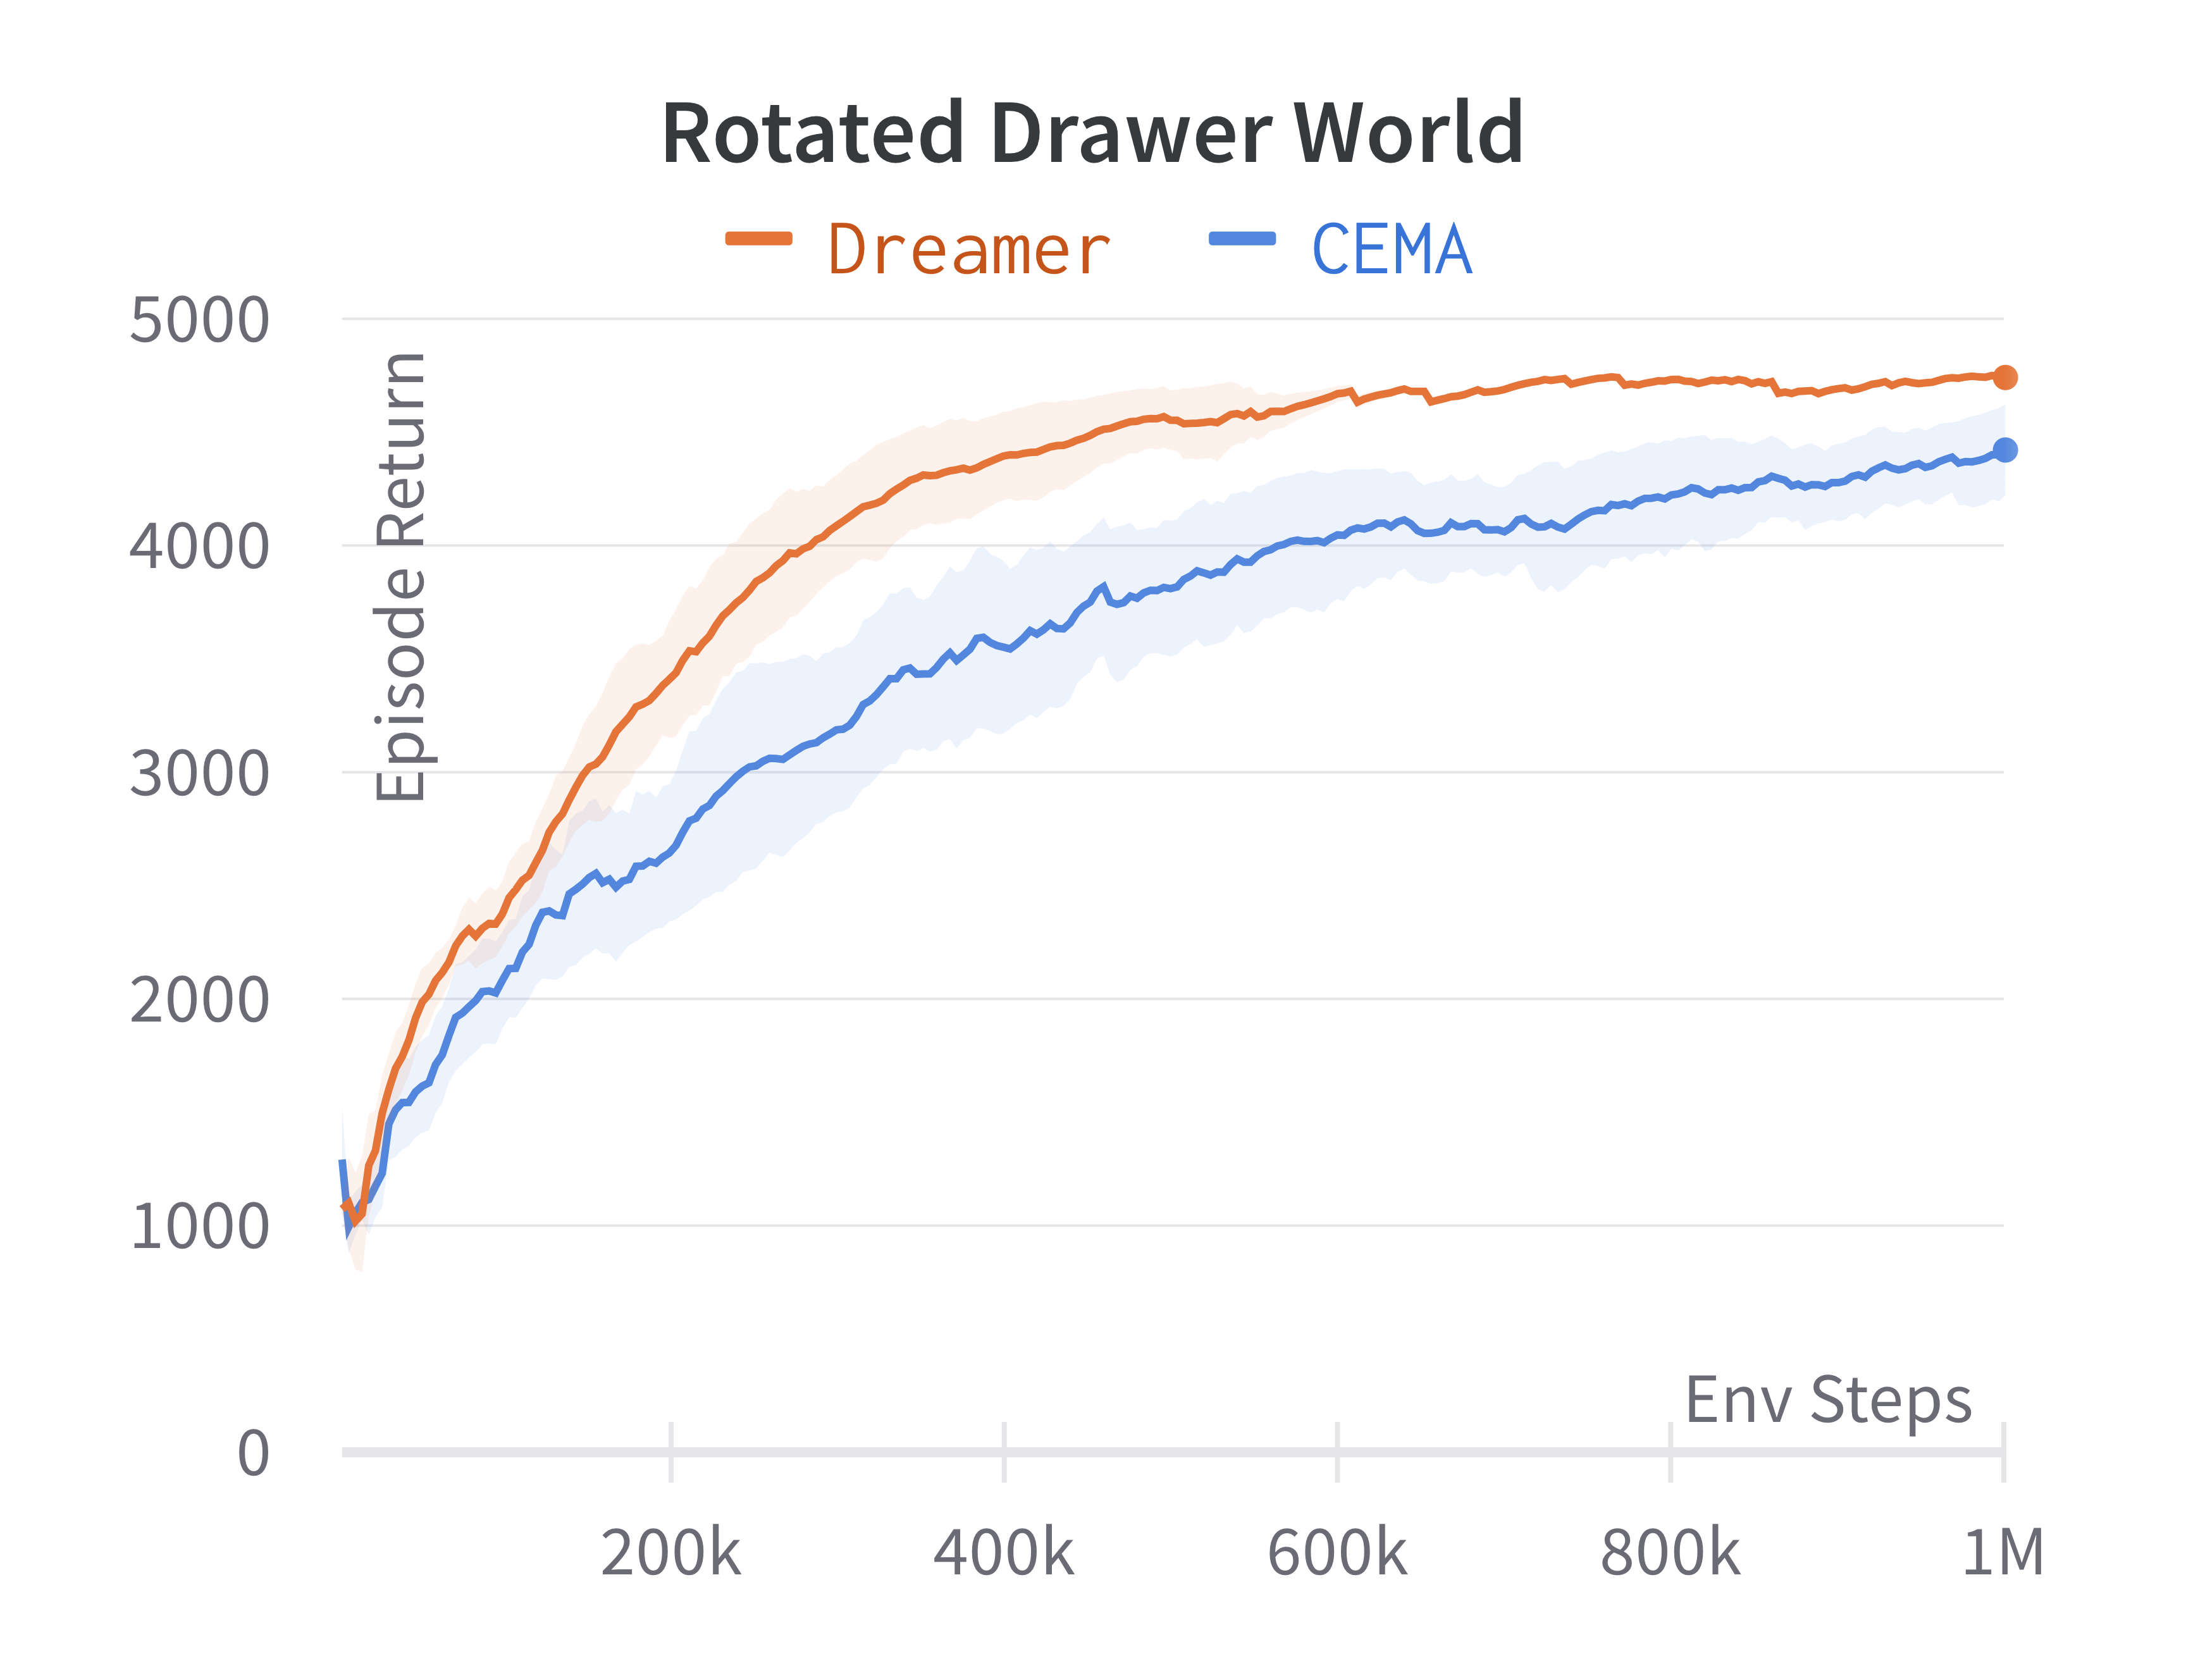
\includegraphics[height=0.5\paperheight]{images/performance/rotated_drawer_train.png}
        \end{subfigure}
      \caption{График наград на тренировочных задачах алгоритмов Dreamer и CEMA. Награды больше $3000$ соответствуют решенной задаче. }
    \end{figure}
\end{column}
\note[item]<1->{The performance of CEMA on training tasks is slightly worse than Dreamer's in terms of task solving speed.}
\hfill
\begin{column}{0.48\linewidth}<2->
    \begin{figure}
        \begin{subfigure}{\linewidth}
          \centering
          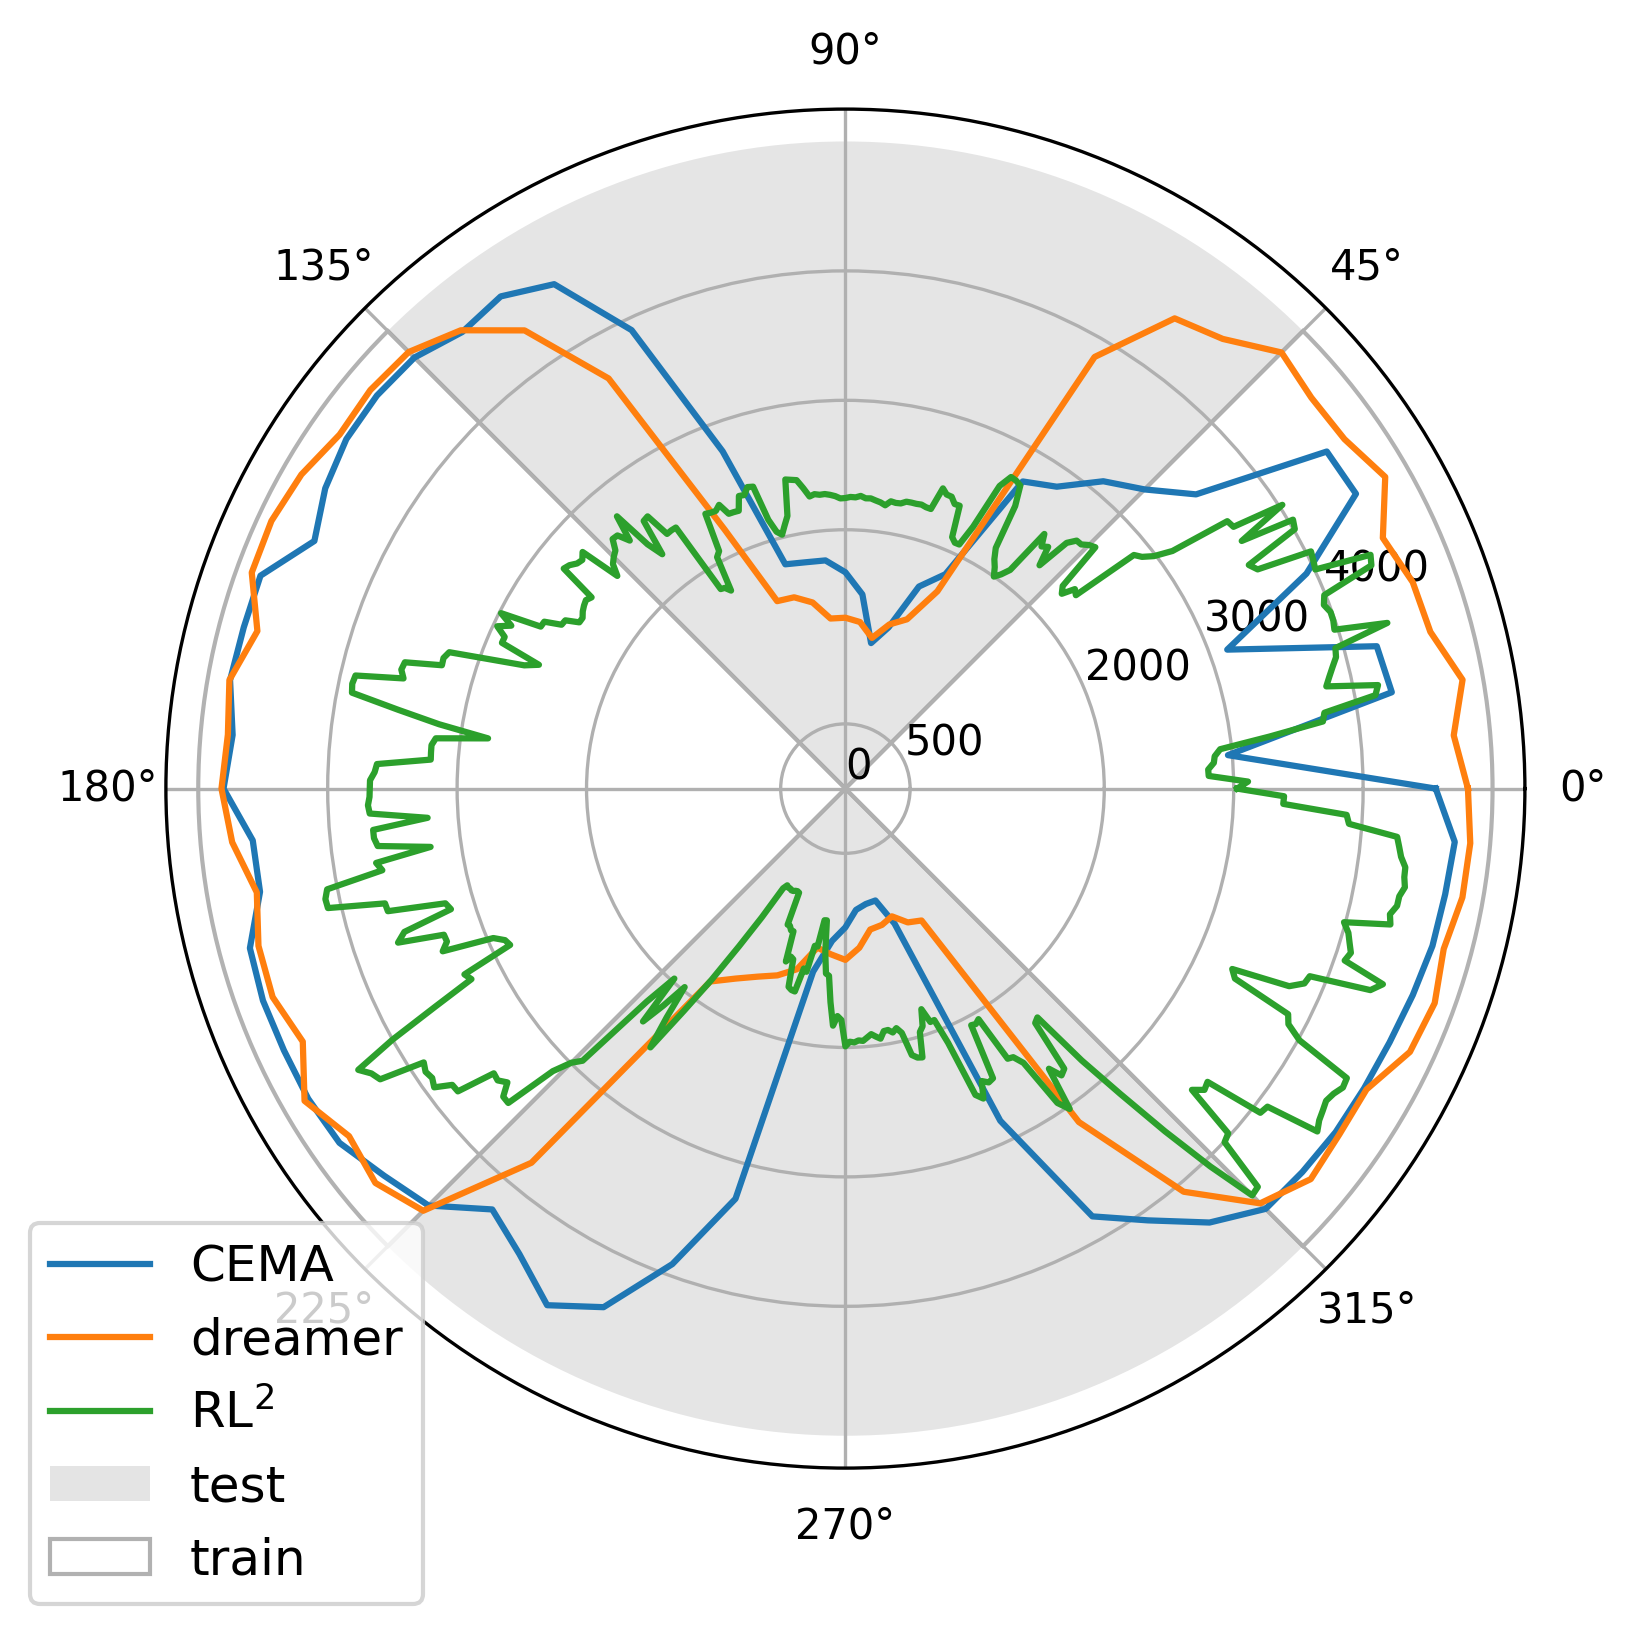
\includegraphics[height=0.5\paperheight]{images/performance/rotated_drawer_eval.png}
          \label{rd_gen_plot}
        \end{subfigure}
      \caption{Результаты работы алгоритмов на каждой задаче. Белые регионы соответствуют тренировочным задачам, синие - тестовым.}
    \end{figure}
\end{column}
\end{columns}
\note[item]<2->{However, its generalization capabilities are better - CEMA is able to solve more OOD tasks than Dreamer}
\end{frame}
\begin{frame}
\frametitle{Эксперимент: Взаимная Информация (MI)}

\onslide<1->{\begin{figure}
    \centering
    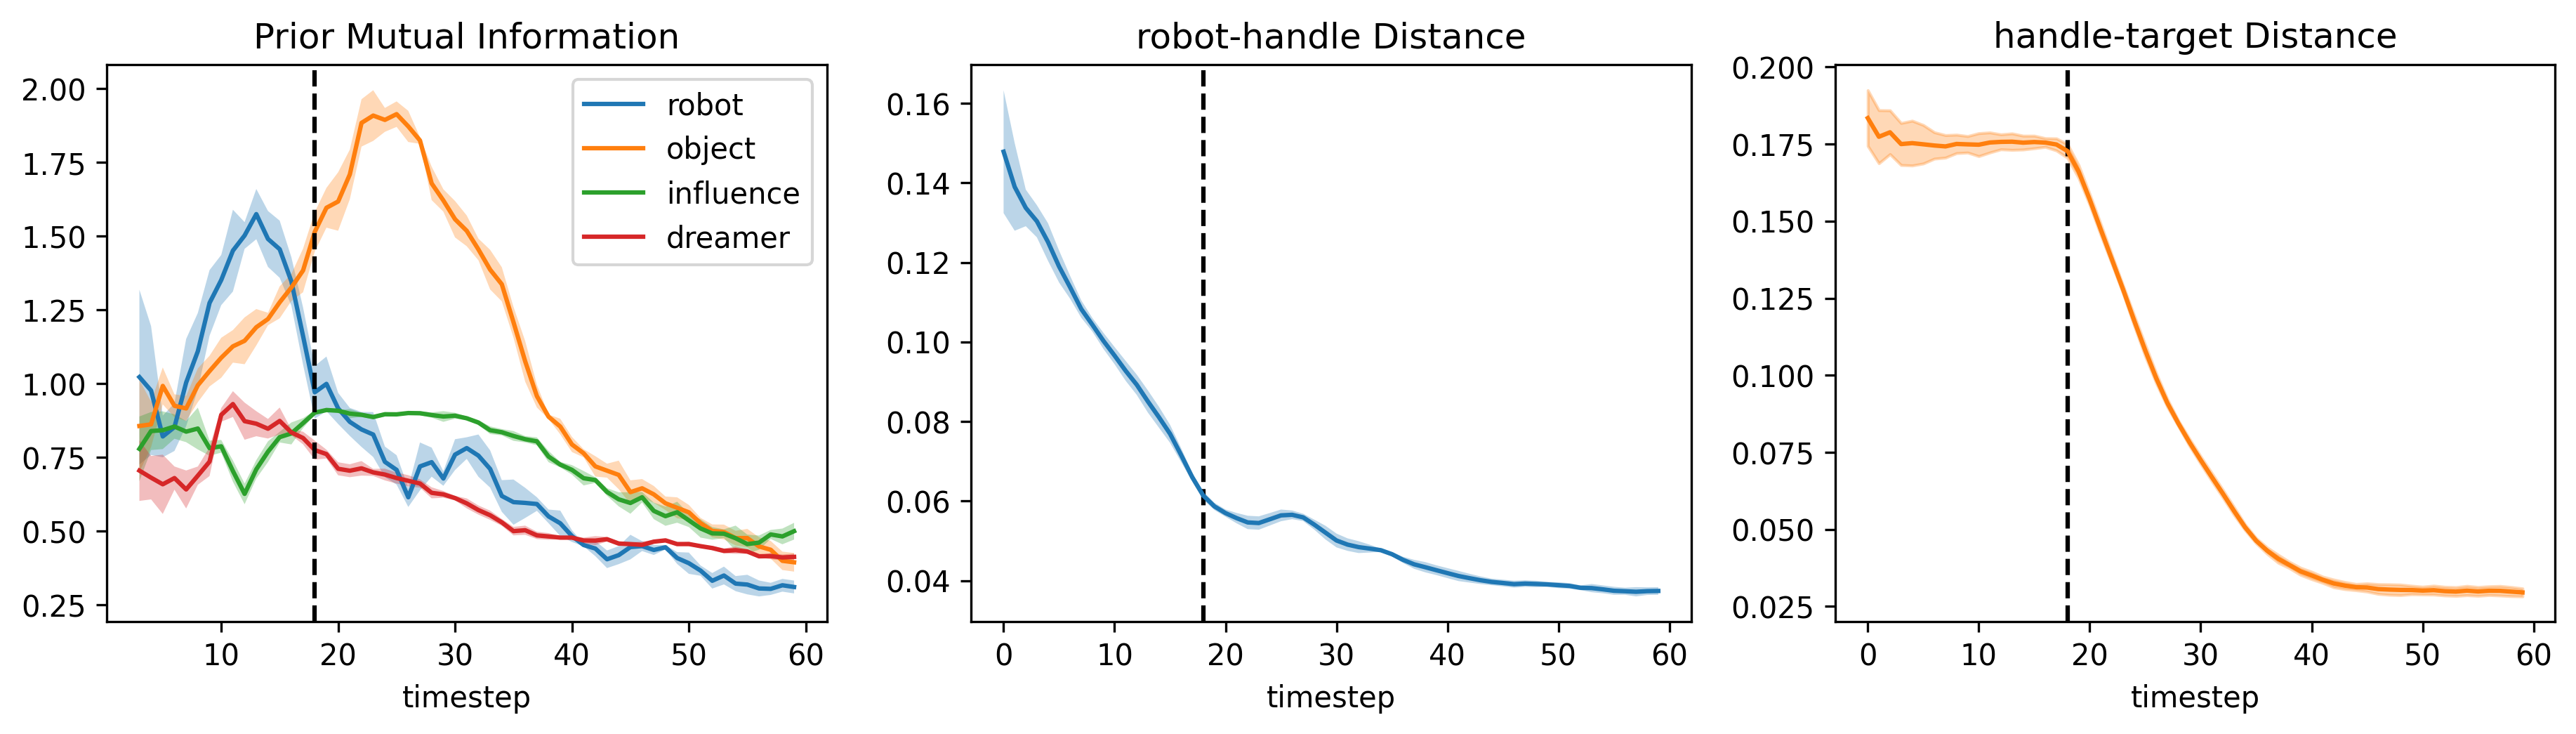
\includegraphics[width=0.95\linewidth]{images/mi_plots/mi_plot.png}
    \caption{Взаимная информацию между входом и выходом различных частей модели мира агента.}
\end{figure}
}
\note[item]<1->{To show how the model can reflect the cause-effect relationships, we study the excitement measure for each conditional distribution, i.e. Conditional Mutual Information between input and output of state distributions. Results show that distributions are activated in bottom-up fashion from robot to object part, propagating influence of actions on object.}
\onslide<2->{\begin{figure}[t]
    \centering
    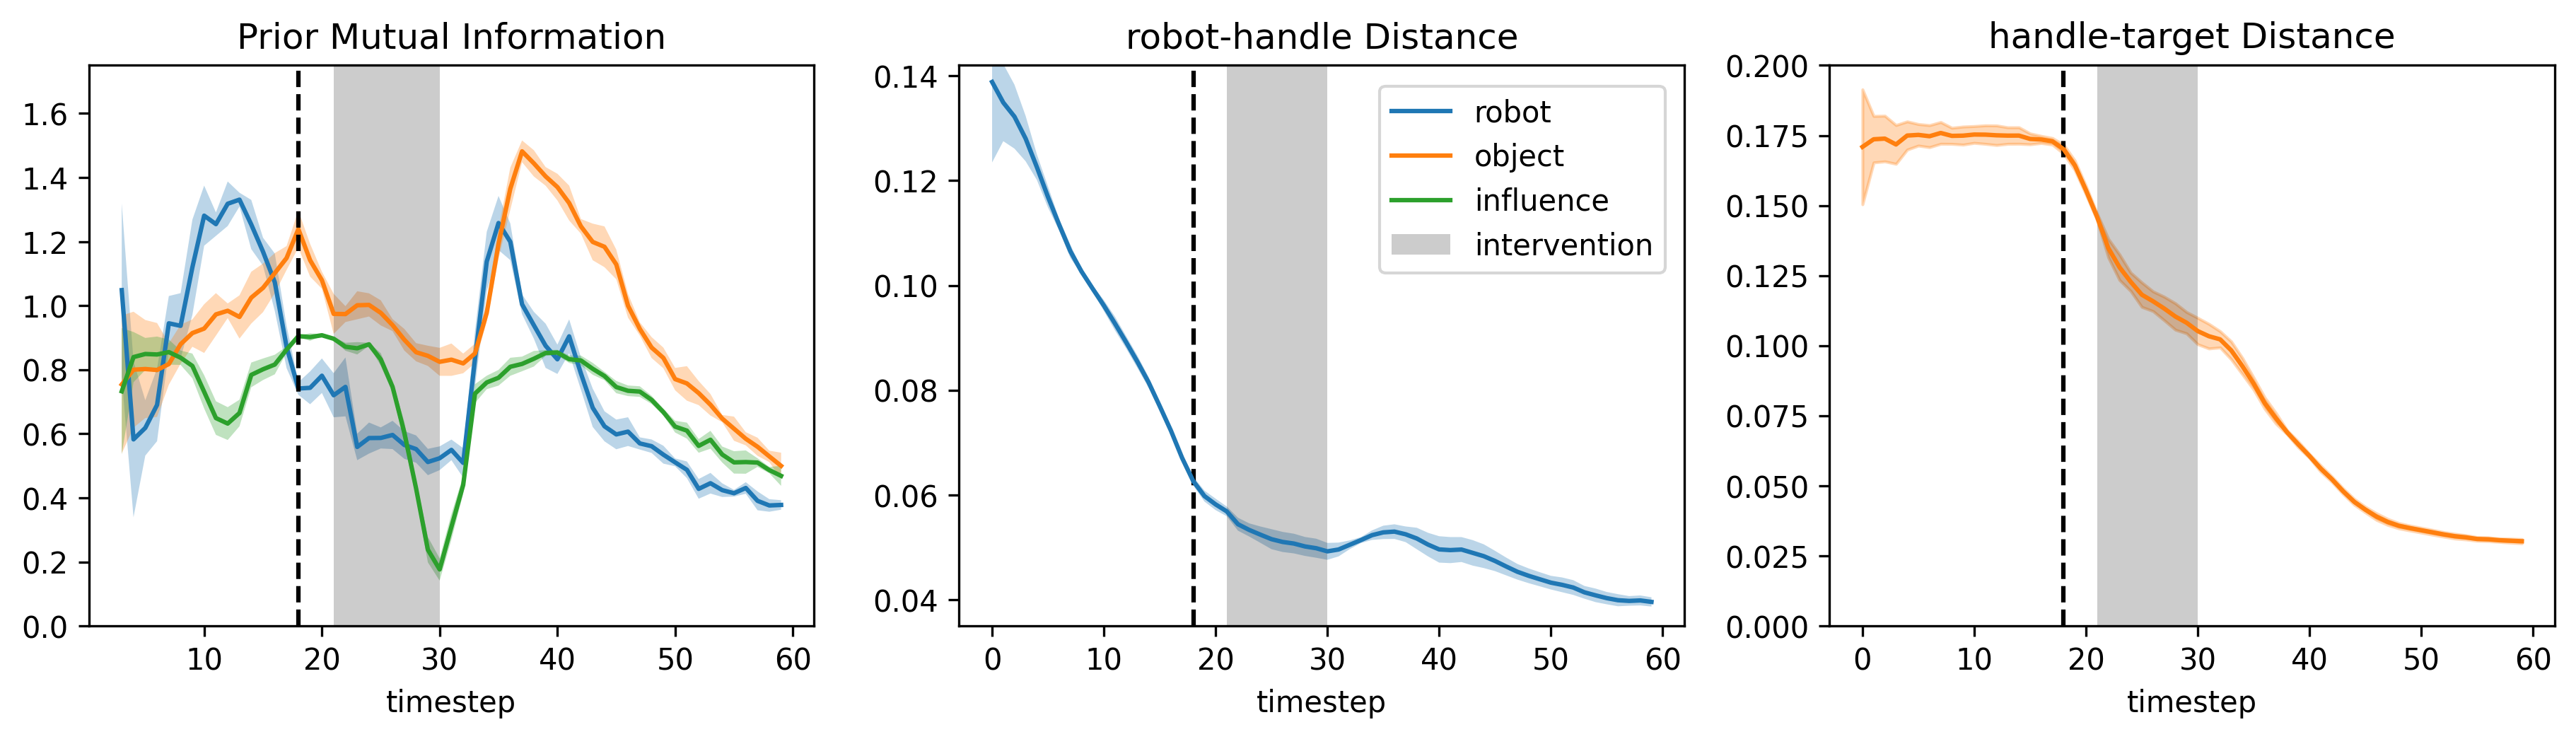
\includegraphics[width=0.95\linewidth]{images/mi_plots/mi_plot_interventions.png}
    \caption{Взаимная информация в условиях искусственного вмешательства в эпизод\footnotemark.}
\end{figure}
}
\onslide<2->{\scriptsize{* В середине открытия ящика, движение всех объектов в среде заморожено путем искусственной вставки нескольких пустых действий.}
}
\note[item]<2->{Also, we conducted the experiment involving stopping the robot hand while it has just begun closing the box. Just after resuming, robot continues to affect the drawer, which results in even faster response in influence state, which, in turn, affects the object state.}
\end{frame}
\begin{frame}
\frametitle{Эксперимент: Causal World, описание среды}

\begin{columns}[t]
\begin{column}{0.33\linewidth}<3->
    Сырое изображение из среды::
    % \begin{itemize}
    %     \item Each observation contains two entities of interest
    %     \item Each entity have its own dynamics
    %     \item Actor can directly affect or have a long-term influence over object
    % \end{itemize}
            \begin{figure}
            \begin{subfigure}{0.8\linewidth}
                \centering
                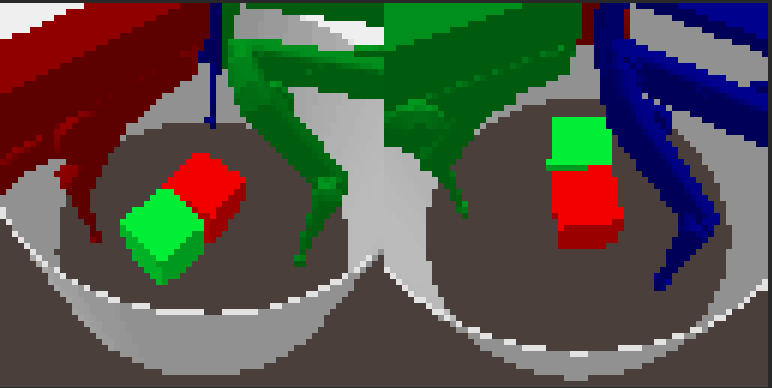
\includegraphics[width=\linewidth]{images/env/causal_world/actual_obs.png}
            \end{subfigure}
            \end{figure}
\end{column}
\hfill
\begin{column}{0.63\linewidth}<1->
    Пример наблюдений:
    \begin{figure}
    \onslide<1->{\begin{subfigure}{.4\linewidth}
        \centering
            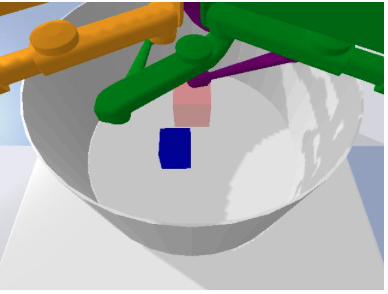
\includegraphics[width=\linewidth]{images/env/causal_world/obs_1.png}
    \end{subfigure}}
    \end{figure}
    \begin{figure}
        \onslide<1->{\begin{subfigure}{.4\linewidth}
            \centering
                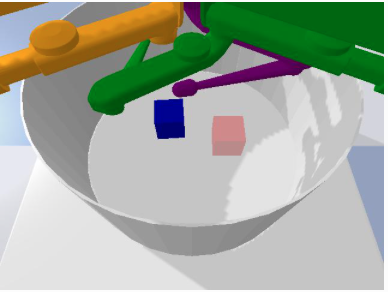
\includegraphics[width=\linewidth]{images/env/causal_world/obs_2.png}
        \end{subfigure}}
        \hspace{3em}%
        \onslide<1->{\begin{subfigure}{.4\linewidth}
            \centering
                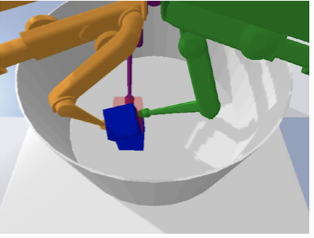
\includegraphics[width=\linewidth]{images/env/causal_world/obs_3.png}
        \end{subfigure}}
    \end{figure}
    
    % Probably not needed
    % \begin{itemize}
    %     \item The task is defined by drawer position
    %     \item Ground truth segmentation masks
    %     \item Out-of-distribution test tasks
    %     \item Single topdown camera for all tasks
    % \end{itemize}
\end{column}
\end{columns}
\note[item]<1->{We built the custom parameterized task environment for evaluating the generalization capabilities of algorithm. It is a drawer, which should be opened by robotic hand.In each specific task, the drawer is fixed.}
\end{frame}
\begin{frame}
\frametitle{Эксперимент: Causal World, результаты}

\begin{columns}[t]
\begin{column}{0.48\linewidth}<1->
    \begin{figure}
        \begin{subfigure}{\linewidth}
        \centering
          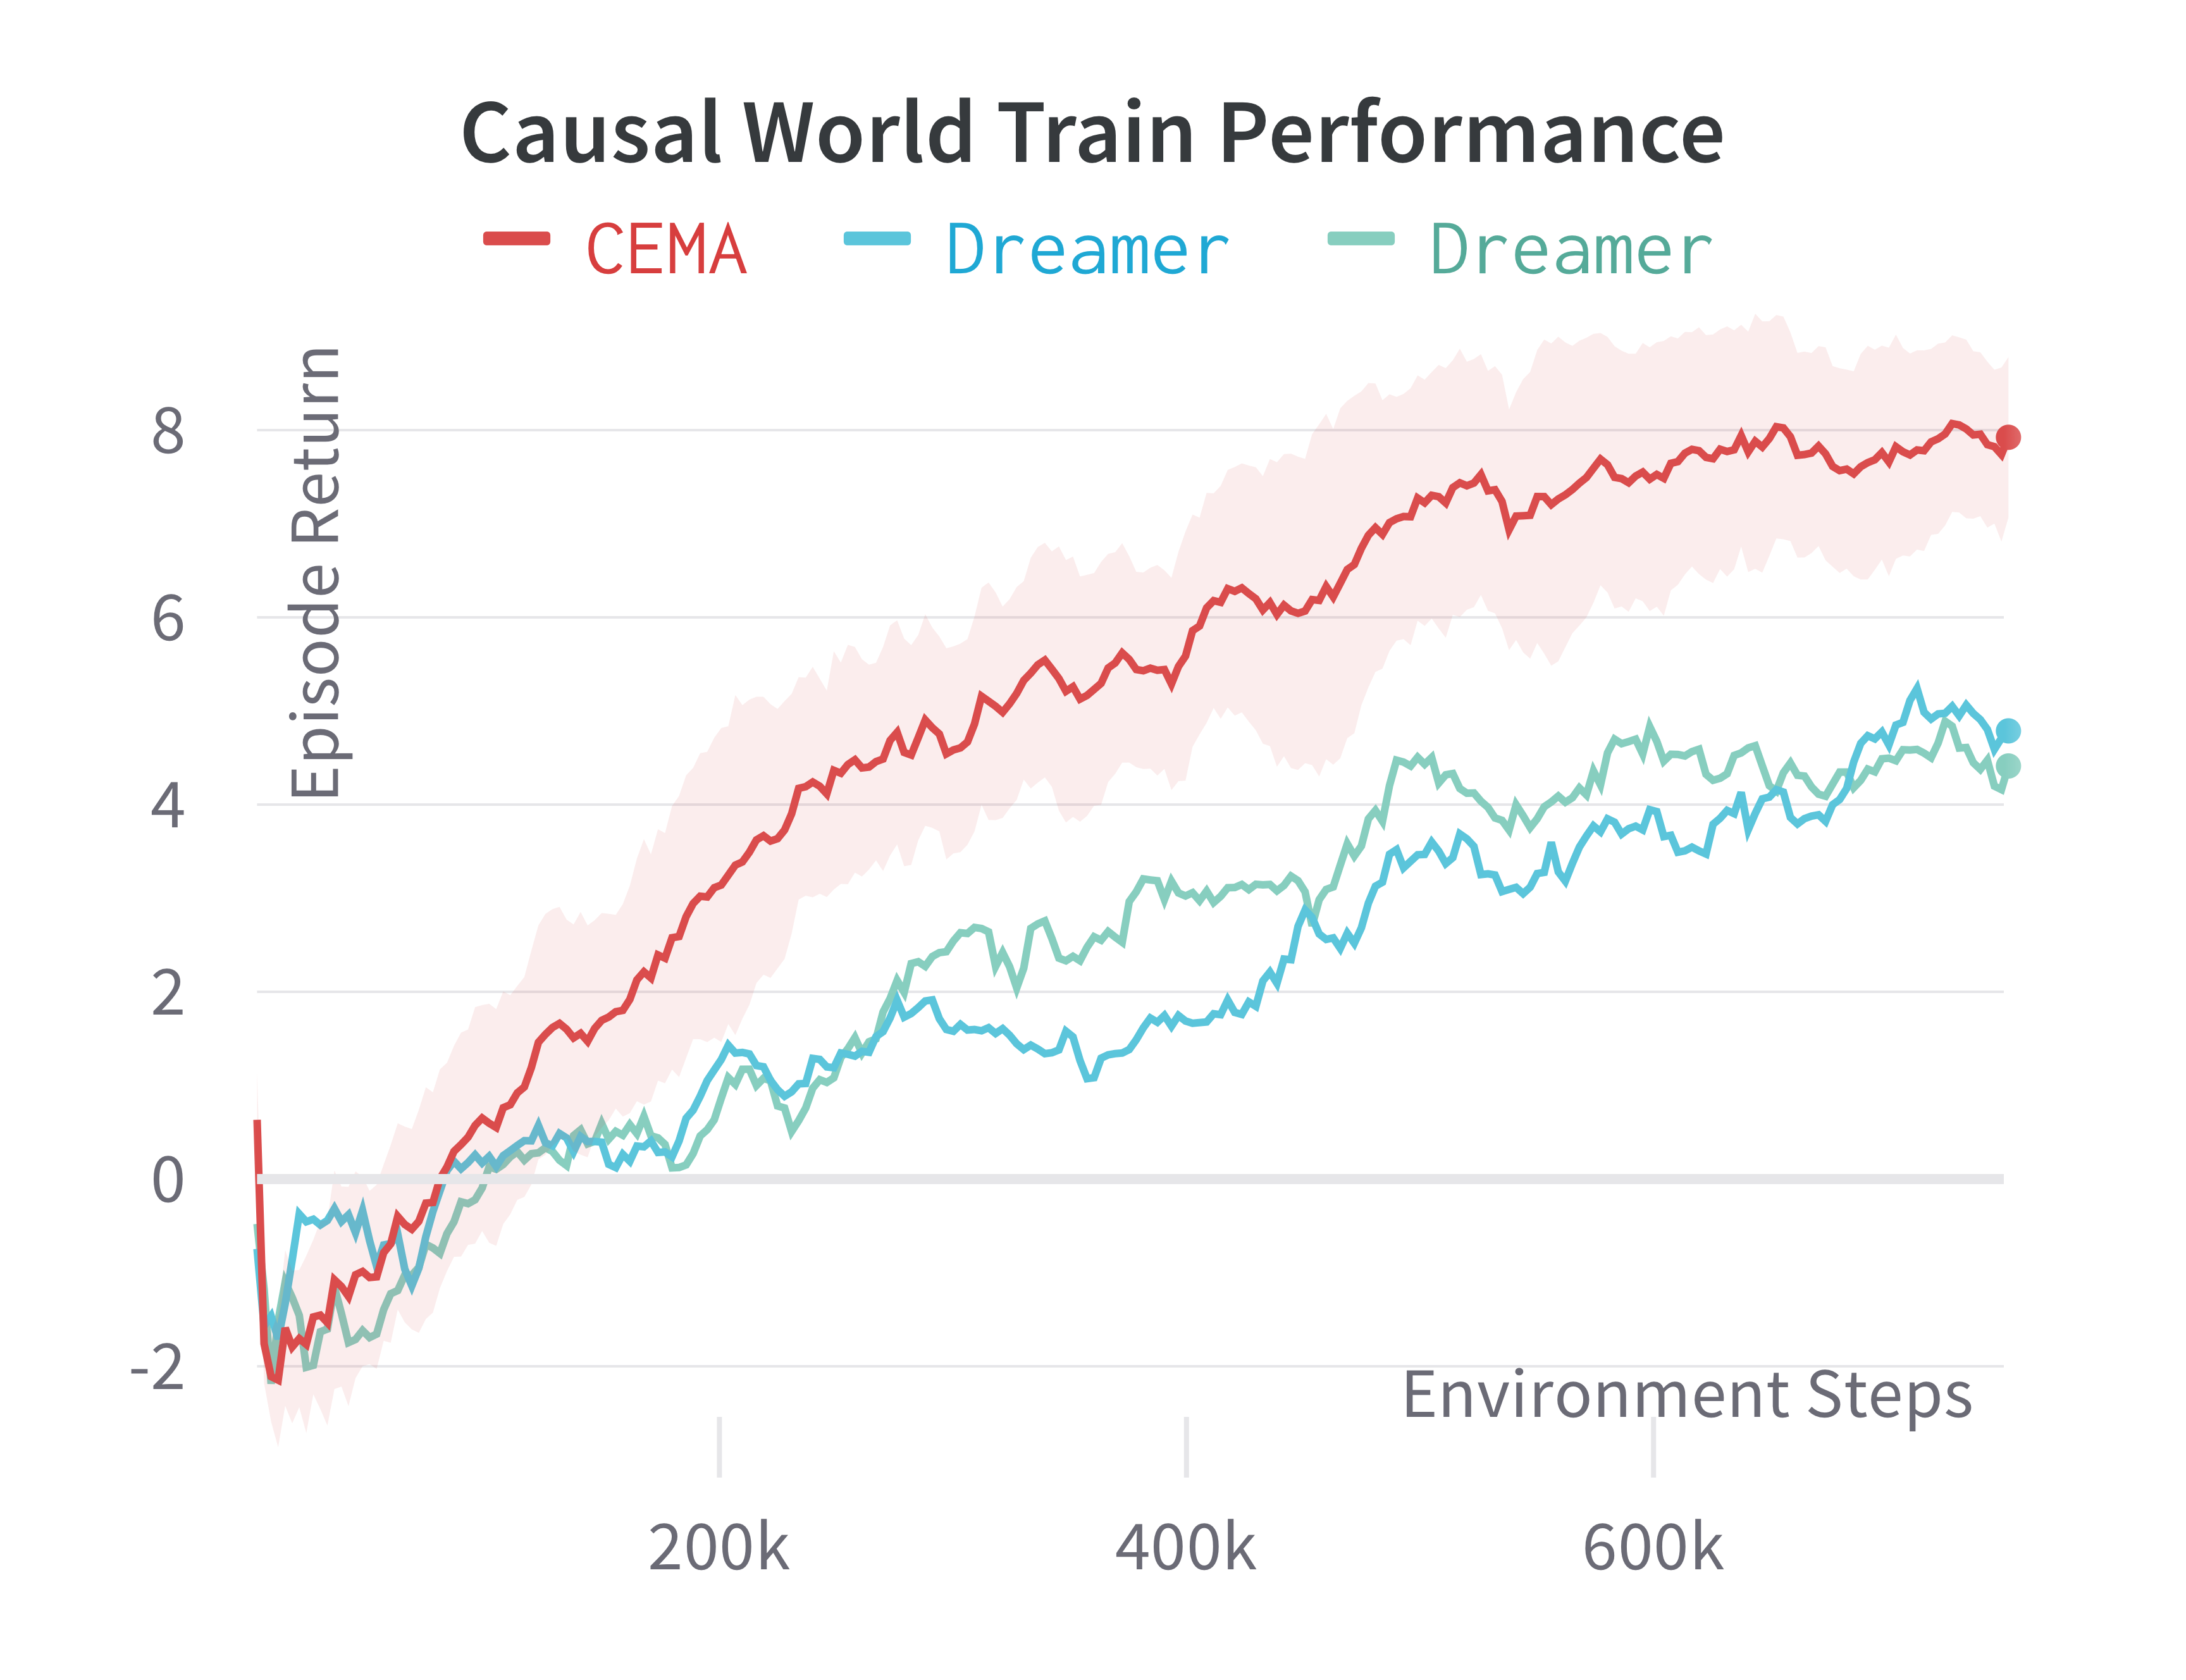
\includegraphics[height=0.5\paperheight]{images/performance/cema_res_cw.png}
        \end{subfigure}
      \caption{График наград на тренировочных задачах алгоритмов Dreamer и CEMA. Представленные награды являются неизмененными наградами среды.}
    \end{figure}
\end{column}
\note[item]<1->{The performance of CEMA on training tasks is slightly worse than Dreamer's in terms of task solving speed.}
\hfill
\begin{column}{0.48\linewidth}<2->
    \begin{figure}
        \begin{subfigure}{\linewidth}
          \centering
          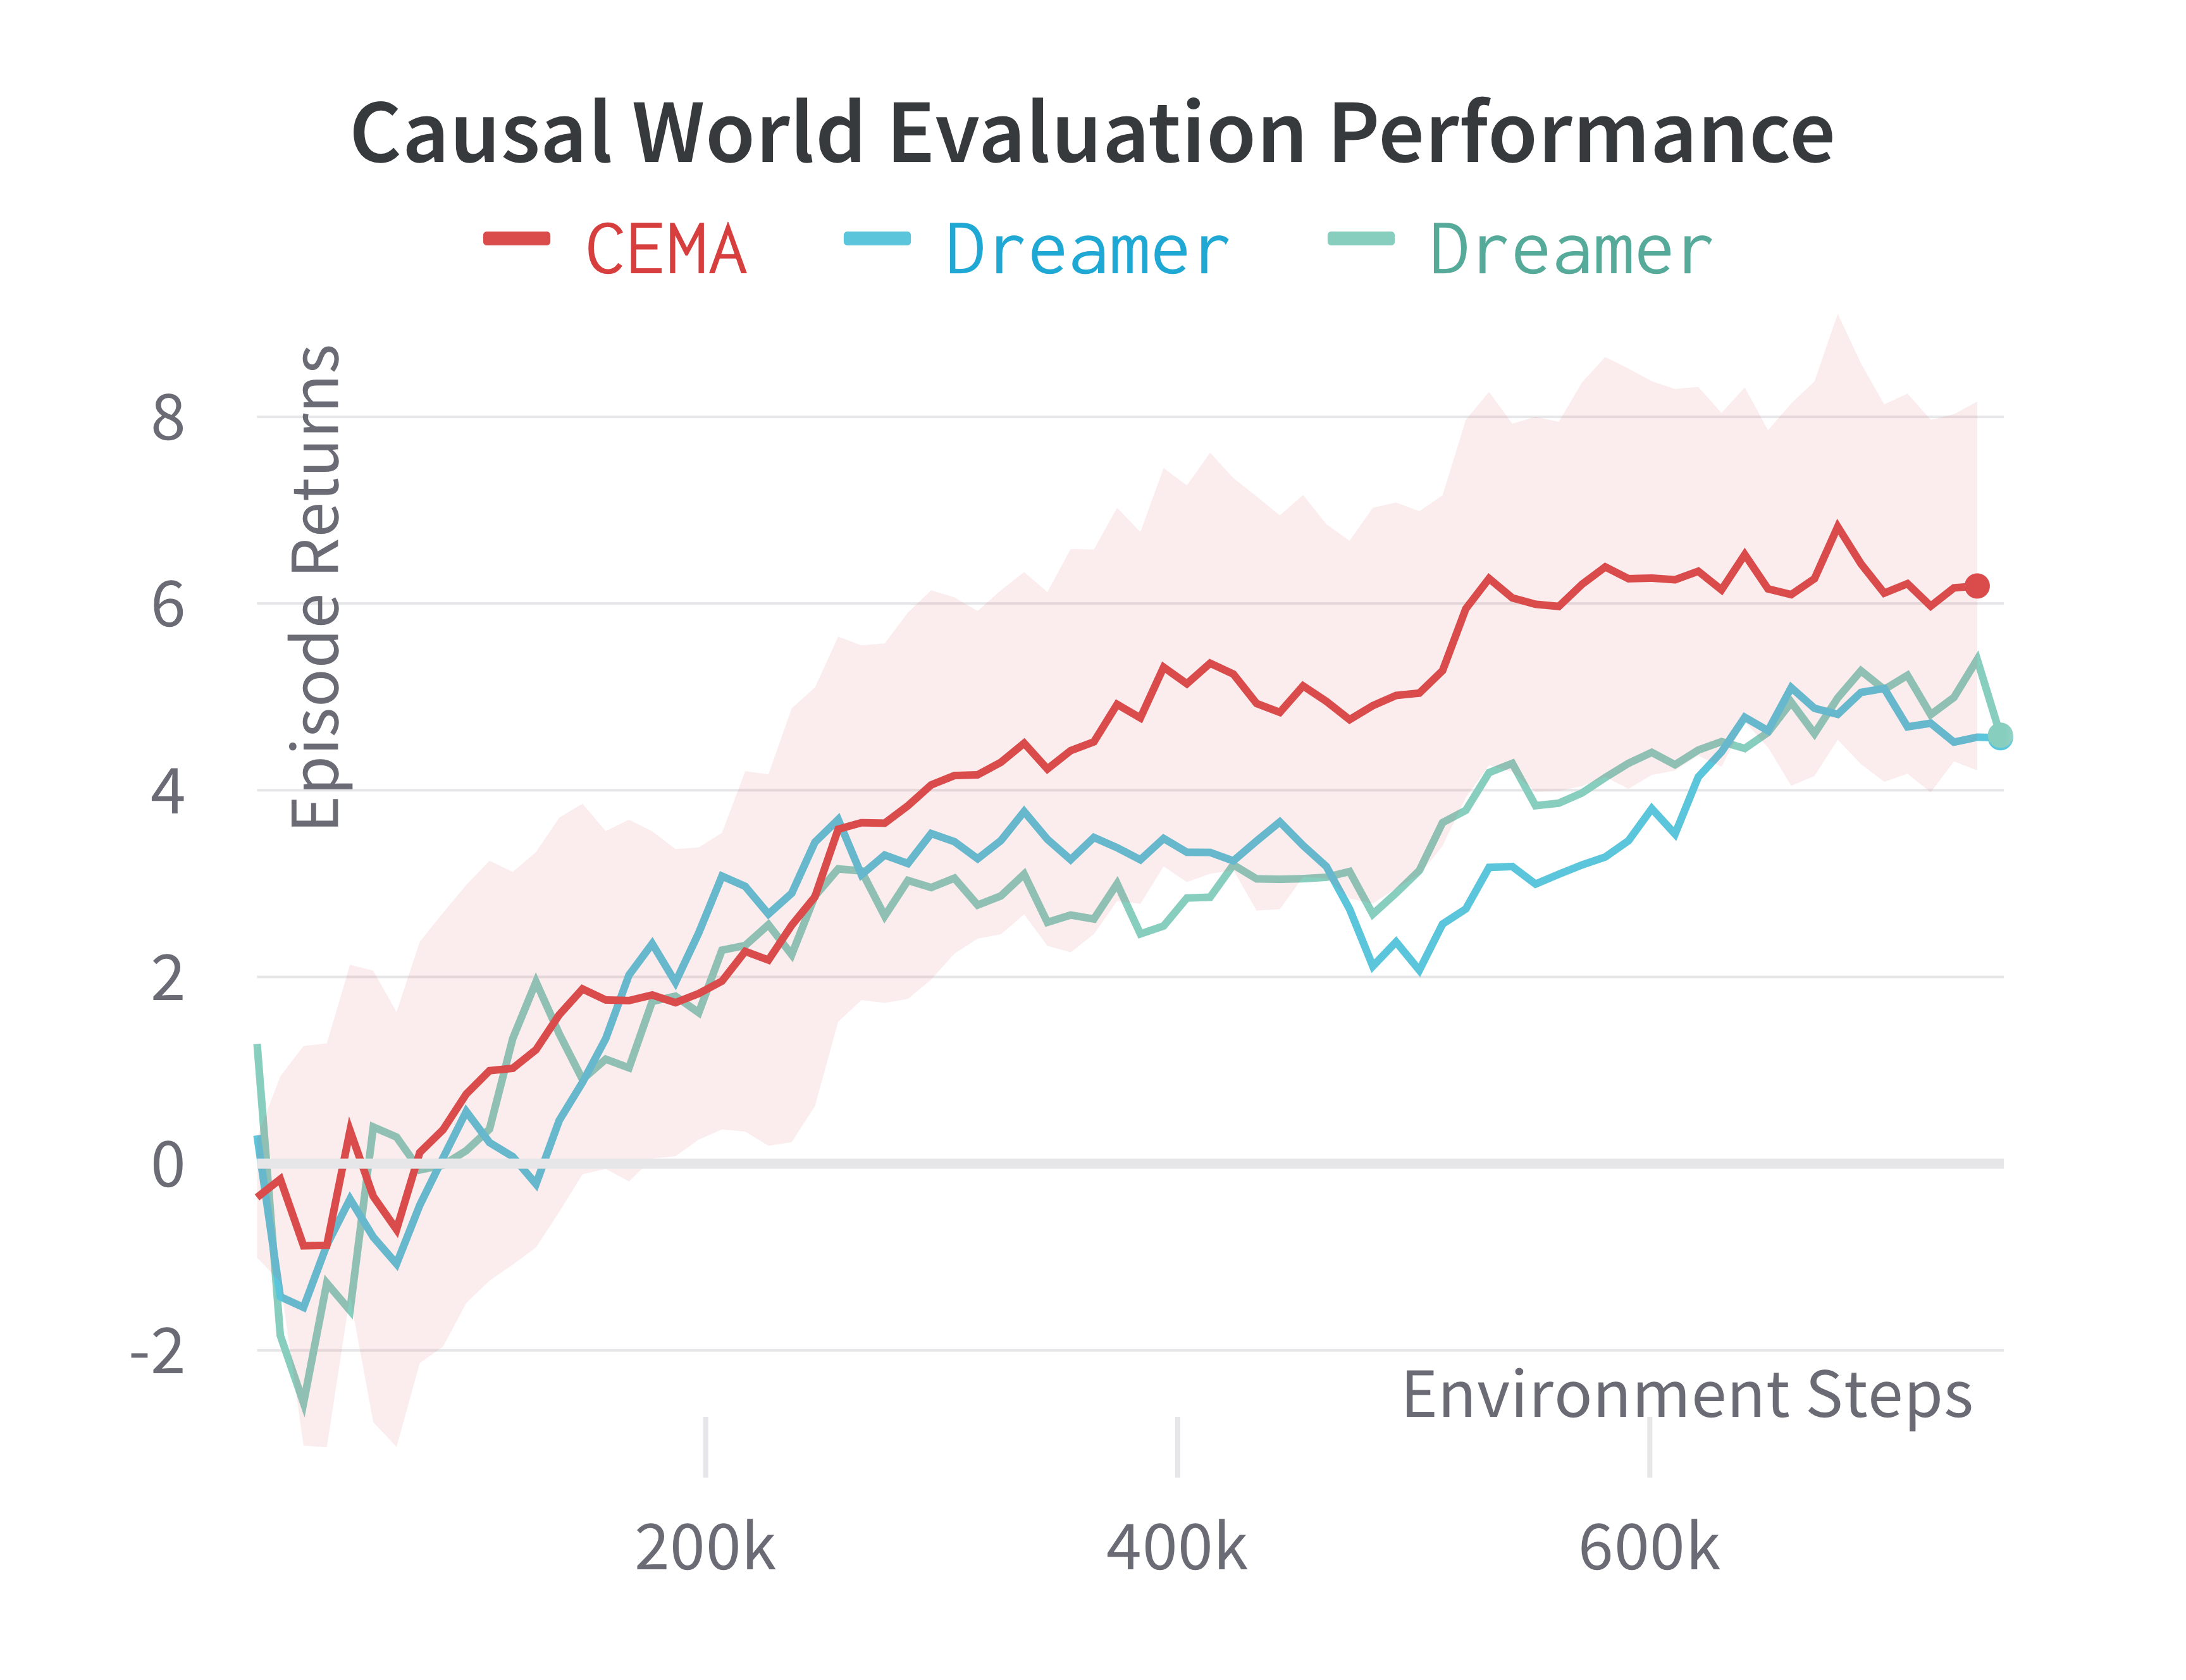
\includegraphics[height=0.5\paperheight]{images/performance/cema_eval_cw.png}
          \label{cw_gen_plot}
        \end{subfigure}
      \caption{Сравнение результатов работы алгоритма на тестовых задачах.}
    \end{figure}
\end{column}
\end{columns}
\note[item]<2->{However, its generalization capabilities are better - CEMA is able to solve more OOD tasks than Dreamer}
\end{frame}
\begin{frame}
\frametitle{Публикации}
\begin{itemize}
    \item \textbf{Принято:} Artem Zholus, Yaroslav Ivchenkov и Aleksandr Panov.
“Factorized World Models for Learning Causal Relationships”. В: ICLR2022
Workshop on the Elements of Reasoning: Objects, Structure and
Causality. 2022. 
    \item \textbf{Отправлено:} Artem Zholus, Yaroslav Ivchenkov, Aleksandr Panov ``Casual Factorized World Models in Model-based Reinforcement Learning''. NeurIPS 2022 (under review)
\end{itemize}

\end{frame}
\begin{frame}
\begin{centering}
    \vskip5ex plus 1filll
    {
    \usebeamerfont{title page title}
    \usebeamercolor[fg]{titlepage}
    \inserttitle\\[1.5ex]
    }
    {
    \usebeamerfont{title page}
    \usebeamercolor[fg]{titlepage}
    Код доступен по адресу:\\[2ex]
    }
    {
    \usebeamerfont{title page author}
    \usebeamercolor[fg]{frametitle}
    \href{https://github.com/artemZholus/generalization_with_world_models}{github.com/artemZholus/generalization\_with\_world\_models}\\[10ex]
    }
    {
    \usebeamerfont{title page title}
    \usebeamercolor[fg]{titlepage}
    Спасибо за внимание!\\[2ex]
    }
    \vskip0pt plus 1filll
\end{centering}
\end{frame}
\note{If you're interested in our model, you can find paper, code and presentation slides in our GitHub repository. Thank you!}
% TODO: make references correct
% \begin{frame}[allowframebreaks]
    
    \frametitle{References}
    % \bibliographystyle{acm} 
    \printbibliography

\end{frame}

% \begin{frame}{A slide title}

  \begin{itemize}
    \item A bulleted item
    \item Another item
      \begin{itemize}
        \item With sub-bullets
        \item And another, with some \textbf{bold} text
      \end{itemize}
    \item And another, at the top level, with \textit{italic} text
  \end{itemize}

  \note{
    Here's a note for this slide.
  }

\end{frame}

% \begin{frame}{A 50-50 split slide}

  \begin{columns}
    \begin{column}{0.5\linewidth}
      \begin{itemize}
        \item This side has a bullet
        \item And another bullet, with text that wraps if it's long
      \end{itemize}
    \end{column}
    \begin{column}{0.5\linewidth}
      \begin{figure}
        \centering
        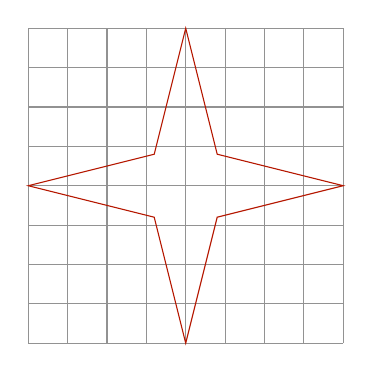
\begin{tikzpicture}[scale=2]
          \draw[step=0.25cm,color=gray] (-1,-1) grid (1,1);
          \draw[color=red] (1,0) -- (0.2,0.2) -- (0,1) -- (-0.2,0.2) -- (-1,0)
          -- (-0.2,-0.2) -- (0,-1) -- (0.2,-0.2) -- cycle;
        \end{tikzpicture}
        \caption{A figure caption}
      \end{figure}
    \end{column}
  \end{columns}

  \note{
    This slide has notes too.
  }

\end{frame}

% \begin{frame}{Full-slide figure}

  \begin{figure}
    \centering
    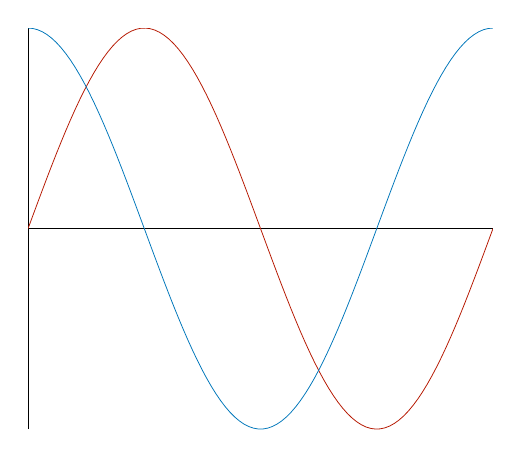
\begin{tikzpicture}[scale=0.7]
      \begin{axis}[
          scale only axis,
          no markers,
          domain=0:2*pi,
          samples=100,
          axis lines=center,
          axis line style={-},
          ticks=none]
        \addplot[red] {sin(deg(x))};
        \addplot[blue] {cos(deg(x))};
      \end{axis}
    \end{tikzpicture}
    \caption{The figure's caption}
  \end{figure}


\end{frame}

% \begin{frame}{A slide with centered text}

  \begin{center}
    Some statement that is centered.
  \end{center}

  \vspace{2ex}
  \begin{center}
    \scriptsize (a small note)
  \end{center}

\end{frame}

% \begin{frame}[fragile]{A slide with some code}

	\begin{columns}
		\begin{column}{0.5\linewidth}
			\footnotesize
			\begin{Verbatim}[commandchars=\\\{\}]
/* some code */
def foo(x):
  return x**0.5 + 2*x

\color{blue}/* some can be highlighted */
\color{blue}foo(3)
      \end{Verbatim}
    \end{column}
    \begin{column}{0.5\linewidth}
      {\color{red} Some explanatory text, in red, with some \texttt{monospace} text.}
      There might be some math, too:

      $$\sqrt{x} + 2x$$
    \end{column}
  \end{columns}

\end{frame}

% \begin{frame}{A slide with some bracketed text}

	\begin{itemize}
		\item Some statement {\color{gray} [Some citation]}
		\item Another statement {\color{gray} [Another citation]}
		\item A final statement {\color{gray} [The last citation]}
	\end{itemize}

	\vspace{3ex}
	\begin{center}
		\scriptsize (a small note)
	\end{center}

\end{frame}


% \begin{frame}{A slide with some text and a link}

  \begin{itemize}
    \item This slide has some text along with a link
      \begin{itemize}
        \item \textbf{Some bold text}: followed by an explanation
        \item \textbf{More bold text}: followed by more text
      \end{itemize}
    \item Another bullet, with sub-bullets
      \begin{itemize}
        \item A sub-bullet
        \item Another sub-bullet, with more text
      \end{itemize}
  \end{itemize}

  \vspace{2ex}
  \begin{center}
    \color{blue} \href{https://github.com/anishathalye/auriga}{github.com/anishathalye/auriga}
  \end{center}

\end{frame}


\end{document}
